% Para definir o tipo de documento, descomente apenas
% uma das linhas "\documentclass" abaixo

% comentar uma linha significa colocar "%"
% descomentar uma linha significa remover o "%"

%\documentclass[msc]{on}     % dissertação de mestrado
%\documentclass[dsc]{on}     % tese de doutorado
%\documentclass[dscexam]{on} % exame de qualificação
\documentclass[reportd]{on} % relatório feito durante o doutorado
%\documentclass[reportm]{on} % relatório feito durante o mestrado

% pacotes utilizados
\usepackage[utf8]{inputenc}
\usepackage{amsmath,amssymb}
\usepackage{hyperref}
\usepackage{enumerate} %para gerar listas numeradas
\usepackage{graphicx}  %para figuras eps
\usepackage{float}
\usepackage{subfigure} %para figuras múltimas, com (a), (b), (c), etc.
%\usepackage[colorlinks = true, linkcolor = black, urlcolor  = blue, citecolor = blue, anchorcolor = blue]{hyperref}
\usepackage{url}%acrescenta url´s
\usepackage{indentfirst}
\usepackage{booktabs} % To thicken table lines

% os dois comandos estão com problema e deverão ser
% corrigidos futuramente
%\makelosymbols
%\makeloabbreviations

\begin{document}

  % Título em português
  \title{Apendizado de máquina no reconhecimento de padrões litológicos}
  
  % Título em inglês
  \foreigntitle{Machine learning in the recognition of lithological patterns}
  
  % Autor
  \author{Victor Ribeiro}{Carreira}

  % Orientador(a)
  %\advisor{Dra.}{Nome da orientadora}{Sobrenome}
  \advisor{Dr.}{Cosme F. Neto,}{Ponte}

  % Co-orientadores (pode ser mais de um)
  %\coadvisor{Dra.}{Nome da Co-orientadora}{Sobrenome}
  %\coadvisor{Dr.}{Nome do Co-orientador}{Sobrenome}

  % Examinadores (caso seja um relatório, não modifique as linhas "\examiner")
  \examiner{Dra.}{Nome da Examinadora}{Sobrenome}
  \examiner{Dr.}{Nome do Examinador}{Sobrenome}
  \examiner{Dra.}{Nome da Examinadora}{Sobrenome}
  \examiner{Dr.}{Nome do Examinador}{Sobrenome}
  \examiner{Dra.}{Nome da Examinadora}{Sobrenome}

  % Programa de Pós-Graduação 
  \program{GEO}
  %\program{ASTRO}
  
  % Data (mês e ano)
  \date{09}{2017}

  % Palavras-chave
  \keyword{Primeira palavra-chave}
  \keyword{Segunda palavra-chave}
  \keyword{Terceira palavra-chave}

  \maketitle

  % caso seja um relatório (de exame de qualificação ou não),
  % comente as quatro (4) próximas linhas
  %\frontmatter     % folha de rosto
  %\makecatalog     % ficha catalogŕafica
  %\include{dedic}  % dedicatória
  %\include{thanks} % agradecimentos
  
  %\begin{abstract}

Apresenta-se, neste relatório, o que foi desenvolvido até o presente momento do projeto de doutorado sobre a aplicação da inteligência artificial no reconhecimento de padrões litológicos. Primeiramente, é apresentado a motivação da obra. Posteriormente, é explicado o que vem a ser redes neuronais e ainda apresento trabalhos já publicados e aplicados na área da perfilagem de poços. Em seguia explico os princípios matemáticos envolvidos e apresento a rede escolhida para resolver o problema proposto. Ao final do capítulo $1$, mostro o que vem a ser aprendizado não-supervisionado. O capítulo $2$ esclarece o contexto geológico da área que virá a ser estudada, nas etapas posteriores do projeto, que será a etapa de trabalho com o dado real. No capítulo $3$, é exposto o método que será utilizado ao longo do projeto bem como quais são os seus objetivos. O capítulo $4$ ilustra a natureza do dado de \textit{well logging} e apresenta um teste de hipóteses realizado, na rede neuronal. No capítulo $5$, são mostrados os resultados desse teste, para as etapas de treinamento e identificação da rede. Estes testes apontaram que o erro da rede relativo à etapa do treinamento foi de $4\%$. E a estabilização da rede se deu com $1000$ ciclos de treinamento e com custo computacional de $20$ segundos, na compilação do programa.  Por conseguinte, no capítulo $6$, são apresentadas as conclusões dos testes sintéticos. São publicados, no capítulo $7$,  o cronograma de atividades do projeto atualizado seguido pelas referências bibliográficas.      

\end{abstract}

   % resumo em português - deve ser utilizado por todos os tipos de documento
  %\include{abstract} % resumo em inglês - deve ser utilizado por todos os tipos de documento
  \tableofcontents   % sumário - deve ser utilizado por todos os tipos de documento
  \listoffigures     % lista de figuras
  \listoftables      % lista de tabelas

  % os dois comandos estão com problema e deverão ser
  % corrigidos futuramente
  %\printlosymbols
  %\printloabbreviations

  \mainmatter

  % As linhas "\include" abaixo incluem os capítulos no documento e
  % devem ser utilizadas por todos os tipos de documento.
  % Edite os arquivos "chapxx.tex" de acordo com as suas necessidades.
  % No presente documento, são incluídos seis capítulos, mas é possível
  % utilizar quantos capítulos forem necessários.
  \chapter{Introdução}

O ser humano vem usando a sua habilidade de reconhecimento de padrões desde  muito antes do início do processo civilizatório. Grupos de humanos paleolíticos já faziam registro dos padrões migratórios de certos grupos de cervídeos. Durante a aurora da revolução neolítica, nossa capacidade de reconhecimento de padrões foi direcionada para a agricultura com a criação de monumentos que registraram a mudança das estações ao longo do ano.

O cérebro humano evoluiu espantosamente. E no que se refere a quantidade de informação processada, o cérebro possui enorme vantagem em relação a quantidade de informação processada por um computador \citep{Hall2014}. Este não para de funcionar somente porque algumas células morrem. Um computador, por sua vez, não funciona quando há degradação da sua unidade central de processamento \citep{Mao1996}.

O campo do aprendizado de máquina aborda a criação de programas computacionais que automaticamente melhorem a si mesmos através da experiência \citep{Michie1994,Levy1997,MacKay2005}. 

%Tanto a rede neuronal quanto a árvore de decisão despontam como estratégias de solução para a resolução de problemas de reconhecimento de padrões \citep{MacKay2005}.

As Redes Neuronais Artificiais (RNA) são inspiradas em modelos sensoriais do processamento de tarefas realizadas pelo cérebro \citep{Hagan1996}. Uma RNA, portanto pode ser criada através da aplicação de algoritmos matemáticos que imitem a tarefa realizada por um neurônio \citep{Nedjah2016}. Uma rede neuronal artificial possui semelhanças com a rede neuronal \footnote{ Em muitas referências na área  da inteligência artificial usa-se o termo neural ao invés de neuronal, contudo empregar o termo neuronal é um cuidado necessário e deve ser empregado no lugar do termo neural. Isso se deve ao fato de que os primeiros modelos matemáticos foram inspirados nas células e processos presentes no sistema nervoso central e não no sistema em toda a sua completude.  } natural presente no sistema nervoso central, neste o cômputo de informações realizado do cérebro é feito através de uma vasta quantidade de neurônios interconectados \citep{Feldman1988,Poulton2002}. A comunicação entre essas células é realizada através de impulsos elétricos. Estes são transmitidos e recebidos por meio de sinapses nervosas entre axônios e dendritos. As sinapses são estruturas elementares e uma unidade funcional localizada entre dois neurônios \citep{Krogh2008}. 

%Já a árvore de decisão auxilia na predição da classe de um objeto em um estudo com base em um treinamento prévio. Ou seja, funciona como um algoritmo de aprendizado de máquina supervisionado que é basicamente aplicado em problemas de classificação \citep{FreundYoav1999}. Funciona tanto para variáveis categóricas quando para variáveis dependentes. Nesse algoritmo, a população original é dividida em dois ou mais grupos de populações homogêneas \citep{Simard2000}. 

\section{Redes Neuronais Artificiais}

\citet{McCulloch1943} redigem o trabalho pioneiro onde foi modelado um neurônio cuja resposta dependia do \textit{input}\footnote{Valor de entrada} que provinha de outros neurônios e do peso utilizado.  Já \citet{Rosenblatt1962} cria a teoria de convergência do \textit{Perceptron} onde ele prova que modelos de neurônios possuem propriedades similares ao cérebro humano \citep{Kanal2001}. Neste sentido as rede neuronais artificiais podem realizar performasses sofisticadas no reconhecimento de padrões, mesmo se alguns neurônios forem destruídos \citep{Levy1997}. \citet{Minsky1969} demonstraram que \textit{Perceptrons} somente resolvem uma classe muito limitada de problemas que podem ser linearizados.

Os primeiros artigos sobre redes neuronais em geofísica datam de $1989$ e são focalizados basicamente na eficiência da RNA diante de dados distintos e como preparar esse dado para inserí-lo na RNA e posteriormente interpretá-lo. As redes neuronais artificiais foram usualmente treinadas com dados sintéticos e depois testados em dados reais. Contudo, hoje é comum usar dados reais para treinar a rede \citep{Adibifard2014}. Embora, ambas as abordagens sejam aceitas. O foco a partir de $1995$ até o presente relaciona-se a algumas aplicações específicas, tais como caracterização de reservatórios e na integração de dados associado a uma interpretação compreensiva, ao contrário de uma aplicação isolada \citep{Poulton2002}. 

No problema específicos de poços, um passo importante é a identificação de topo e base de camadas que podem ser associadas com mudanças das propriedades petrofísicas \citep{Saljooghi2014}. Algoritmos baseados em derivadas nas curvas de log não identificam camadas muito finas, ou ruído \citep{Zhang1999}. \citet{Chakravarthy1999} consegue através do uso da função radial localizar os limites de camadas em alta definição em dados de log de indução (HDIL). Já \citet{Benaouda1999} consegue classificar tipos litológicos em poços parcialmente desmoronados através do uso da rede neuronal com propagação de erro e mudanças de classes a medida que prossegue a análise. \citet{Gloaguen2017} levanta a questão da importância relativa das propriedades físicas, em dados de perfilagem de poços,  para a tomada de decisão da rede neuronal.

O neurônio de \citet{McCulloch1943} propõe um limite binário para a criação de um modelo. Este neurônio artificial registra uma soma de pesos de $n$ sinais de entrada, $x_{j}$, $j=1,2,3,...,n$, e fornece um \textit{output}\footnote{Valor de saída} de $1$ caso esta soma esteja acima do limite $u$. Caso contrário o \textit{output} é $0$. Matematicamente essa relação pode ser descrita de acordo com a Eq. \ref{Eq.neuronio-McCulloch}:

\begin{eqnarray}
y=\theta \left( \sum^{n}_{j=1} w_{j} x_{j} -u \right)
\label{Eq.neuronio-McCulloch}
\end{eqnarray}

Onde $\theta$ é o passo dado na posição $0$, $w_{j}$ é chamada sinapse-peso associado a um $j_{esimo}$ \textit{input}. A título de simplificação a função limite\footnote{Genericamente chamada de função de ativação} $u$ é considerada um outro peso $w_{0}=-u$ anexado a um neurônio com um \textit{input} constante $x_{0}=1$. Pesos positivos correspondem a uma sinapse \textbf{excitatória}, enquanto pesos negativos correspondem a uma sinapse \textbf{inibitória}. Este modelo contém uma série de simplificações que não refletem o verdadeiro comportamento dos neurônios biológicos \citep{Mao1996}.  

Derivações do neurônio de \citet{McCulloch1943} na escolha das funções de ativação. Uma função largamente utilizada é a função sigmóide, que exibe uma suavização dos \textit{outputs} a medida que o valor da função diminui \citep{Mao1996,Misra2010}. Essa função de ativação pode ser expressa de acordo com a Eq. \ref{f.sigmoide}:

\begin{eqnarray}
g(x)=1/(1+e^{-\beta x})
\label{f.sigmoide}
\end{eqnarray}

Onde $\beta$ é o parâmetro de inclinação. A Fig. \ref{Esquematico de McCulloch} ilustra a sequência lógica da operação de uma RNA para um neurônio simples de McCulloch-Pitts. 
\\
\begin{figure}[H]
	\centering
	\setlength{\fboxsep}{8pt}
	\setlength{\fboxrule}{0.1pt}
	\fbox{
	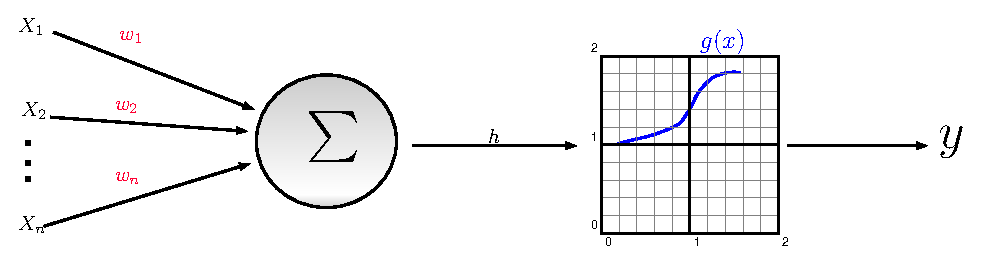
\includegraphics[scale=0.7]{Imagens/McCulloch.eps}
	}
	\caption{Modelo esquemático de um neurônio de McCulloch-Pitts. Onde $x_{1}, x_{2}, ..., x_{n}$ são os \textit{inputs}, $w_{1}, w_{2}, ..., w_{n}$ são os pesos, h é o treino, $g(x)$ é a função de ativação, e $y$ é o \textit{output}.}
	\label{Esquematico de McCulloch}
\end{figure}

Mais de $50$ tipos de redes neuronais artificiais tem sido criadas até o ano de $2014$ \citep{Saljooghi2014}.


\section{A Rede de Kohonen}

Neste trabalho, foi utilizada a rede de kohonen. Esta rede neuronal tem como importante característica ser uma rede com aprendizado não-supervisionado, portanto o espaço solução de saída da rede não é conhecido. 

A localização espacial de um neurônio da saída em um mapa topológico
corresponde a um domínio ou característica particular do dado retirado do espaço de entrada. E estas entradas são mapeadas de forma ordenada, a exemplo dos mapas cito-arqueturais do córtex cerebral.

Neste processo de identificação de padrões a redundância torna-se impreterível,
pois o neurônio da camada de saída que apresentar a maior resposta terá os seus
pesos ajustados. Além disso, o peso dos neurônios vizinhos também serão
ajustados em menor intensidade ao comparados com o neurônio vencedor.

Isto implica que os neurônios devem estar posicionados em um arranjo geométrico
adequado. Esta teoria é baseada na suposição de que as células nervosas
corticais estão organizadas anatomicamente em relação aos estímulos que recebem
dos sensores aos quais estão ligadas \citep{Artero2009}.

Este modelo exige a definição de vizinhança entre neurônios de forma geométrica. Alguns arranjos são comumente utilizados, como por exemplo, os arranjos triangulares, hexagonal, retangulares, etc.

No caso de arranjos retangulares, diferentes vizinhanças de um neurônio
$N_{i,j}$ podem ser configuradas em quartetos, diagonais e octetos. 

A Fig. \ref{hiperplano} ilustra o arranjo retangular e as vizinhanças, em quartetos, adotado neste trabalho. 

\begin{figure}[H]
	\centering
	\setlength{\fboxsep}{8pt}
	\setlength{\fboxrule}{0.1pt}
	\fbox{
		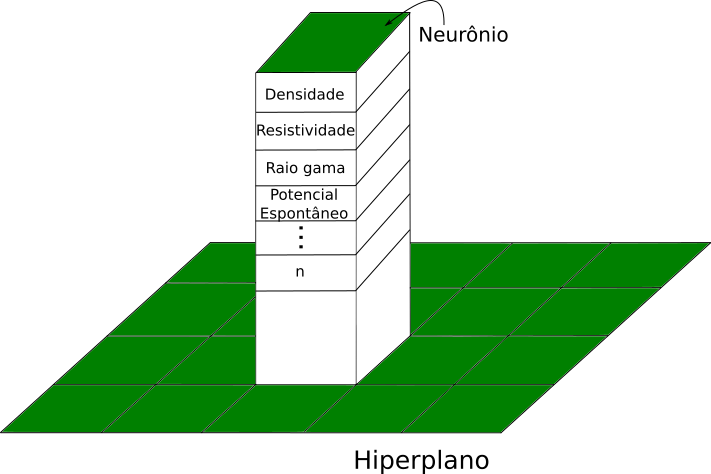
\includegraphics[scale=0.5]{Imagens/hiperplano.png}
	}
	\caption{Neurônio e suas vizinhanças}
	\label{hiperplano}
\end{figure}

O conceito de vizinhança representa uma competição pelo melhor aprendizado e o ajuste do vencedor e da sua vizinhança é um estímulo para que os neurônios ao redor do vencedor também melhorem.

Durante a etapa de treinamento é identificado o neurônio que tem os parâmetros de entrada mais parecidos com os valores dos pesos. Este procedimento é realizado via cálculo da distância euclidiana, Eq. \ref{euclidiana}, entre o parâmetro de entrada $x(t)$ e o peso $w_{i,j}$.

\begin{eqnarray}
d(t)= \sum^{n}_{i=1}[x(t)-w_{i,j}(t)]^{2}
\label{euclidiana}
\end{eqnarray}

A etapa de treinamento da rede se dá por um ajuste de pesos entre os neurônios através do cálculo do menor valor de $d(t)$ na iteração $t$, caracterizando assim o neurônio que passar por esse processo de \textit{vencedor}. Esse procedimento ajusta da mesma forma os pesos do neurônio da vizinhança dentro. Os pesos são ajustados co uma fração da diferença entre os \textit{inputs} $x_{i}$ e os pesos $w_{i}$, vide Eq.\ref{ajuste de pesos}.

\begin{equation}
w_{i,j}(t+1)=w_{i,j}(t)+n(t)[x(t)-w_{i,j}]
\label{ajuste de pesos}
\end{equation}

Através deste ajuste continuado de pesos os elementos do conjunto de entrada são reorganizados de tal foma que as classes próximas sejam posicionados umas perto das outras. Isso gera um mapa bi-dimensional denominado na literatura de \textit{mapa auto-organizável}. Este mapa é o análogo matemático mais fiel das áreas especializadas do córtex cerebral que são ilustradas pelo \textit{Homúnculo de Penfield}, \ref{homunculo}.

\section{Redes com aprendizado não-supervisionado}

Nesta categoria de RNA's são apenas inseridos os valores de \textit{input} da rede. Os \textit{output} são definidos pela própria rede que passa por um processo de treinamento não supervionado. As redes que são submetidas a este tipo de treinamento são mais indicadas para tarefas aonde são exigidos agrupamento de dados (\textit{clustering}). Neste processo uma classe deve ser atribuída aos registros da rede observando-se apenas o comportamento de seus atributos, no caso em particular deste trabalho tratam-se de propriedades geofísicas.

Uma rede com treinamento não supervisionado inspira-se no funcionamento do córtex cerebral. Neste modelo biológico, o organismo aprende a realizar alguma tarefa, por meio da identificação de padrões. Por exemplo, ao identificar uma música determinados padrões sonoros que compõe o conjunto harmonioso de notas precisam ser aprendidos antes de serem reconhecidos. Durante este processo, regiões específicas do cérebro vão sendo paulatinamente acionadas. Isto somente é possível, devido conexões específicas que são formadas entre os neurônios
presentes no córtex, Fig. \ref{homunculo}.

Os detalhes dos processos que regulam o córtex ainda não foram totalmente elucidados, contudo é seguro assumir que a primeira representação dos fenômenos de aprendizagem podem ser representados por uma superfície topológica ou mapa auto-organizado. 

\begin{figure}[H]
	\centering
	\setlength{\fboxsep}{8pt}
	\setlength{\fboxrule}{0.1pt}
	\fbox{
		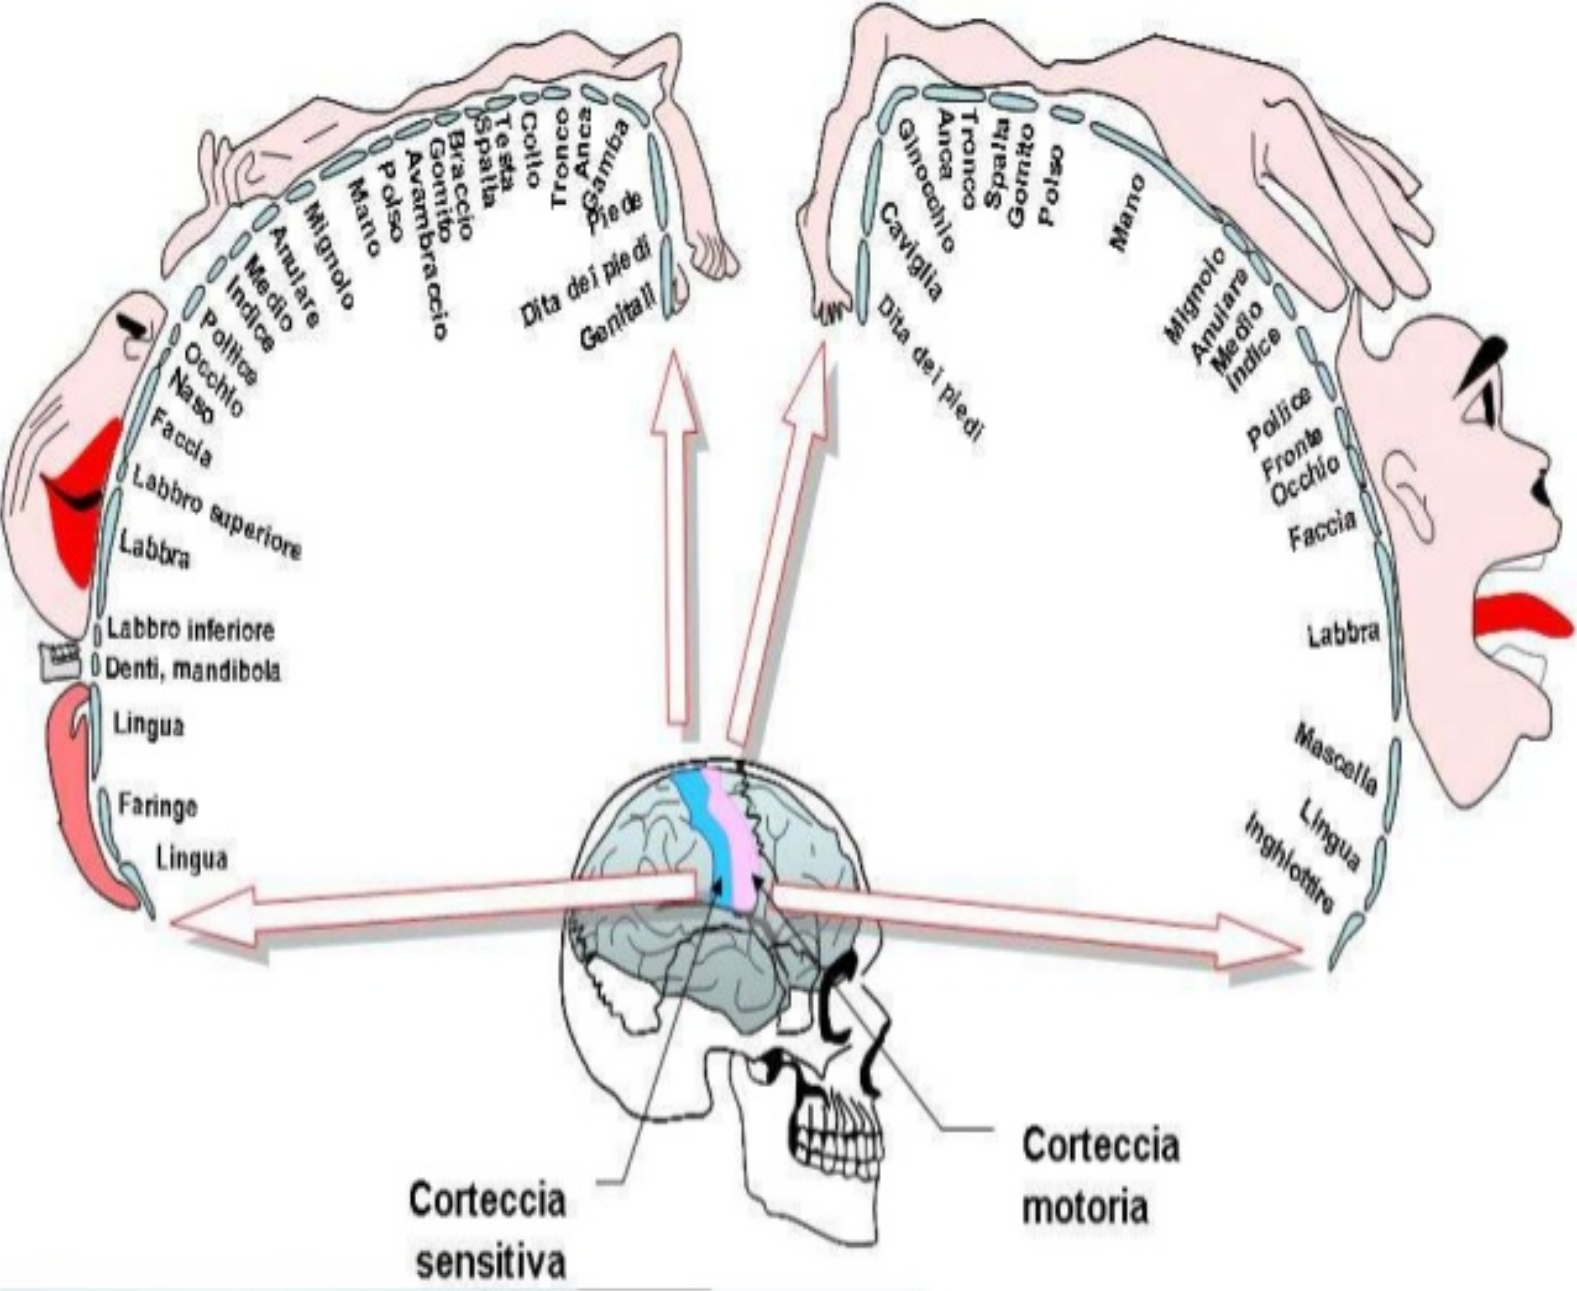
\includegraphics[scale=0.5]{Imagens/homunculo.png}
	}
	\caption{Homúnculo de Penfield.}
	\label{homunculo}
\end{figure}

Um cérebro que sofreu uma comossão grave perde a capacidade de acessar
determinadas zonas do homúnulo responsáveis por atividades específicas. Contudo
o cérebro tem a capacidade de destinar outras regiões para o controle destas
ações que foram previamente perdidas.

Além de casos graves como um acidente o cérebro também perde a capacidade de
aprendizado com o tempo. Em humanos, a capacidade de aprendizado vai da pequena
infância até a puberdade. Após este período, o cérebro passar a reter o que fora
aprendido. Sendo assim o aprendizado é uma função que depende, entre outras
coisas, do tempo.

  \chapter{Contexto Geológico}
A Bacia do Paraná desenvolveu-se sobre uma área de escudo do continente Gondwana Sul e é composta por uma série de núcleos cratônicos, rodeados por vários cinturões móveis e cobertos por bacias molássicas, que foram desenvolvidas durante o ciclo termo-tectônico Brasiliano que se estendeu desde o neoproterozóico até o Ordoviciano. A deformação decorrente deste ciclo teve início entre $700$ Ma e $650$ Ma, sendo que a maior parte das intrusões de granitos que podemos observar na Bacia, situou-se dentro do limite entre o Proterozóico e o Paleozóico (cerca de $570$ Ma) com resfriamento durante o Cambro-Ordoviciano entre $500-450$ Ma \citep{zalan_p._v._tectonica_1987, hawkesworth_tectonic_2000}.

O embasamento que circunda a Bacia do Paraná é dividido em: margem Leste/Sudeste, representado pelas faixas Dom Feliciano e Ribeira ,de idade Brasiliana e de direção NE-SW, separados por um núcleo cratônico designado Rio de La Plata/ Luiz Alves; margem Norte/Nordeste, representada pela faixa Uruaçu, de idade mesoproterozóica, de direção NW e por dois maciços arqueanos (Guaxupé e Goiás) remobilizados durante o ciclo Brasiliano; margem Oeste/Noroeste representada pela faixa de dobramentos Paraguai/Araguaia, também do ciclo Brasiliano, que delimita o extremo da borda Noroeste da Bacia \citep{borghi_2002, hawkesworth_tectonic_2000}.

Dentre os principais grupos de estruturas, nota-se três grupos de lineamentos de direções preferenciais NW-SE, E-W e NE-SW, representando cada um evento termo-tectônico distinto. O conjunto de lineamentos NW-SE são os mais antigos e estão relacionados ao evento  termo-tectônico do Transamazônico, e, as zonas de falhas geológicas associadas a este evento foram reativadas durante o rifteamento do Atlântico Sul, no Cretáceo.  Os lineamentos E-W, tiveram início a partir do Triássico e são paralelos às zonas de fratura oceânica, sugerindo uma ligação com o desenvolvimento do Atlântico Sul. Os lineamentos NE-SW são derivados do evento tremo-tectônico Brasiliano e de seus cinturões móveis associados. Este último conjunto de lineamentos é isento de diques de basalto \citep{milani_outline_1999}. 

O registro estratigráfico da Bacia do Paraná é formado por pacote sedimentar e magmático de espessura máxima em torno de $7000$ m, que coincide geograficamente com o depocentro estrutural da sinéclise e com a calha do rio paraná \citep{milani_orogenias_1998}. O registro estratigráfico da Bacia do Paraná é dividido em seis unidades de ampla escala ou supersequências \citep{Vail_1977} na forma de pacotes rochosos com intervalos temporais de algumas dezenas de milhões de anos de duração e envelopados por superfícies de discordância de caráter inter-regional: Rio Ivaí (Ordoviciano-Siluriano), Paraná (Devoniano), Gondwana I (Carbonífero-Eotriássico), Gondwana II (Meso a Neotriássico), Gondwana III (Neojurássico-Eocretáceo) e Bauru (Neocretáceo). As três primeiras supersequências são representadas por sucessões sedimentares que definem ciclos transgressivos e regressivos ligados às oscilações do nível relativo do mar, durante o Paleozóico, ao passo que as demais correspondem a pacotes de sedimentos continentais com rochas ígneas associadas. As unidades formais da litoestratigrafia, quais sejam os grupos, formações e membros comumente utilizados na descrição do arranjo espacial dos estratos da bacia, inserem-se como elementos particularizados neste arcabouço aloestratigráfico de escala regional \citep{boletim_2007}.

O mapa geológico (Fig. \ref{mapa geologico}) apresenta a extensão e os limites da Bacia do Paraná \citep{Vidotti_2003}.



\begin{figure}[H]
	\centering
	\setlength{\fboxsep}{8pt}
	\setlength{\fboxrule}{0.1pt}
	\fbox{
		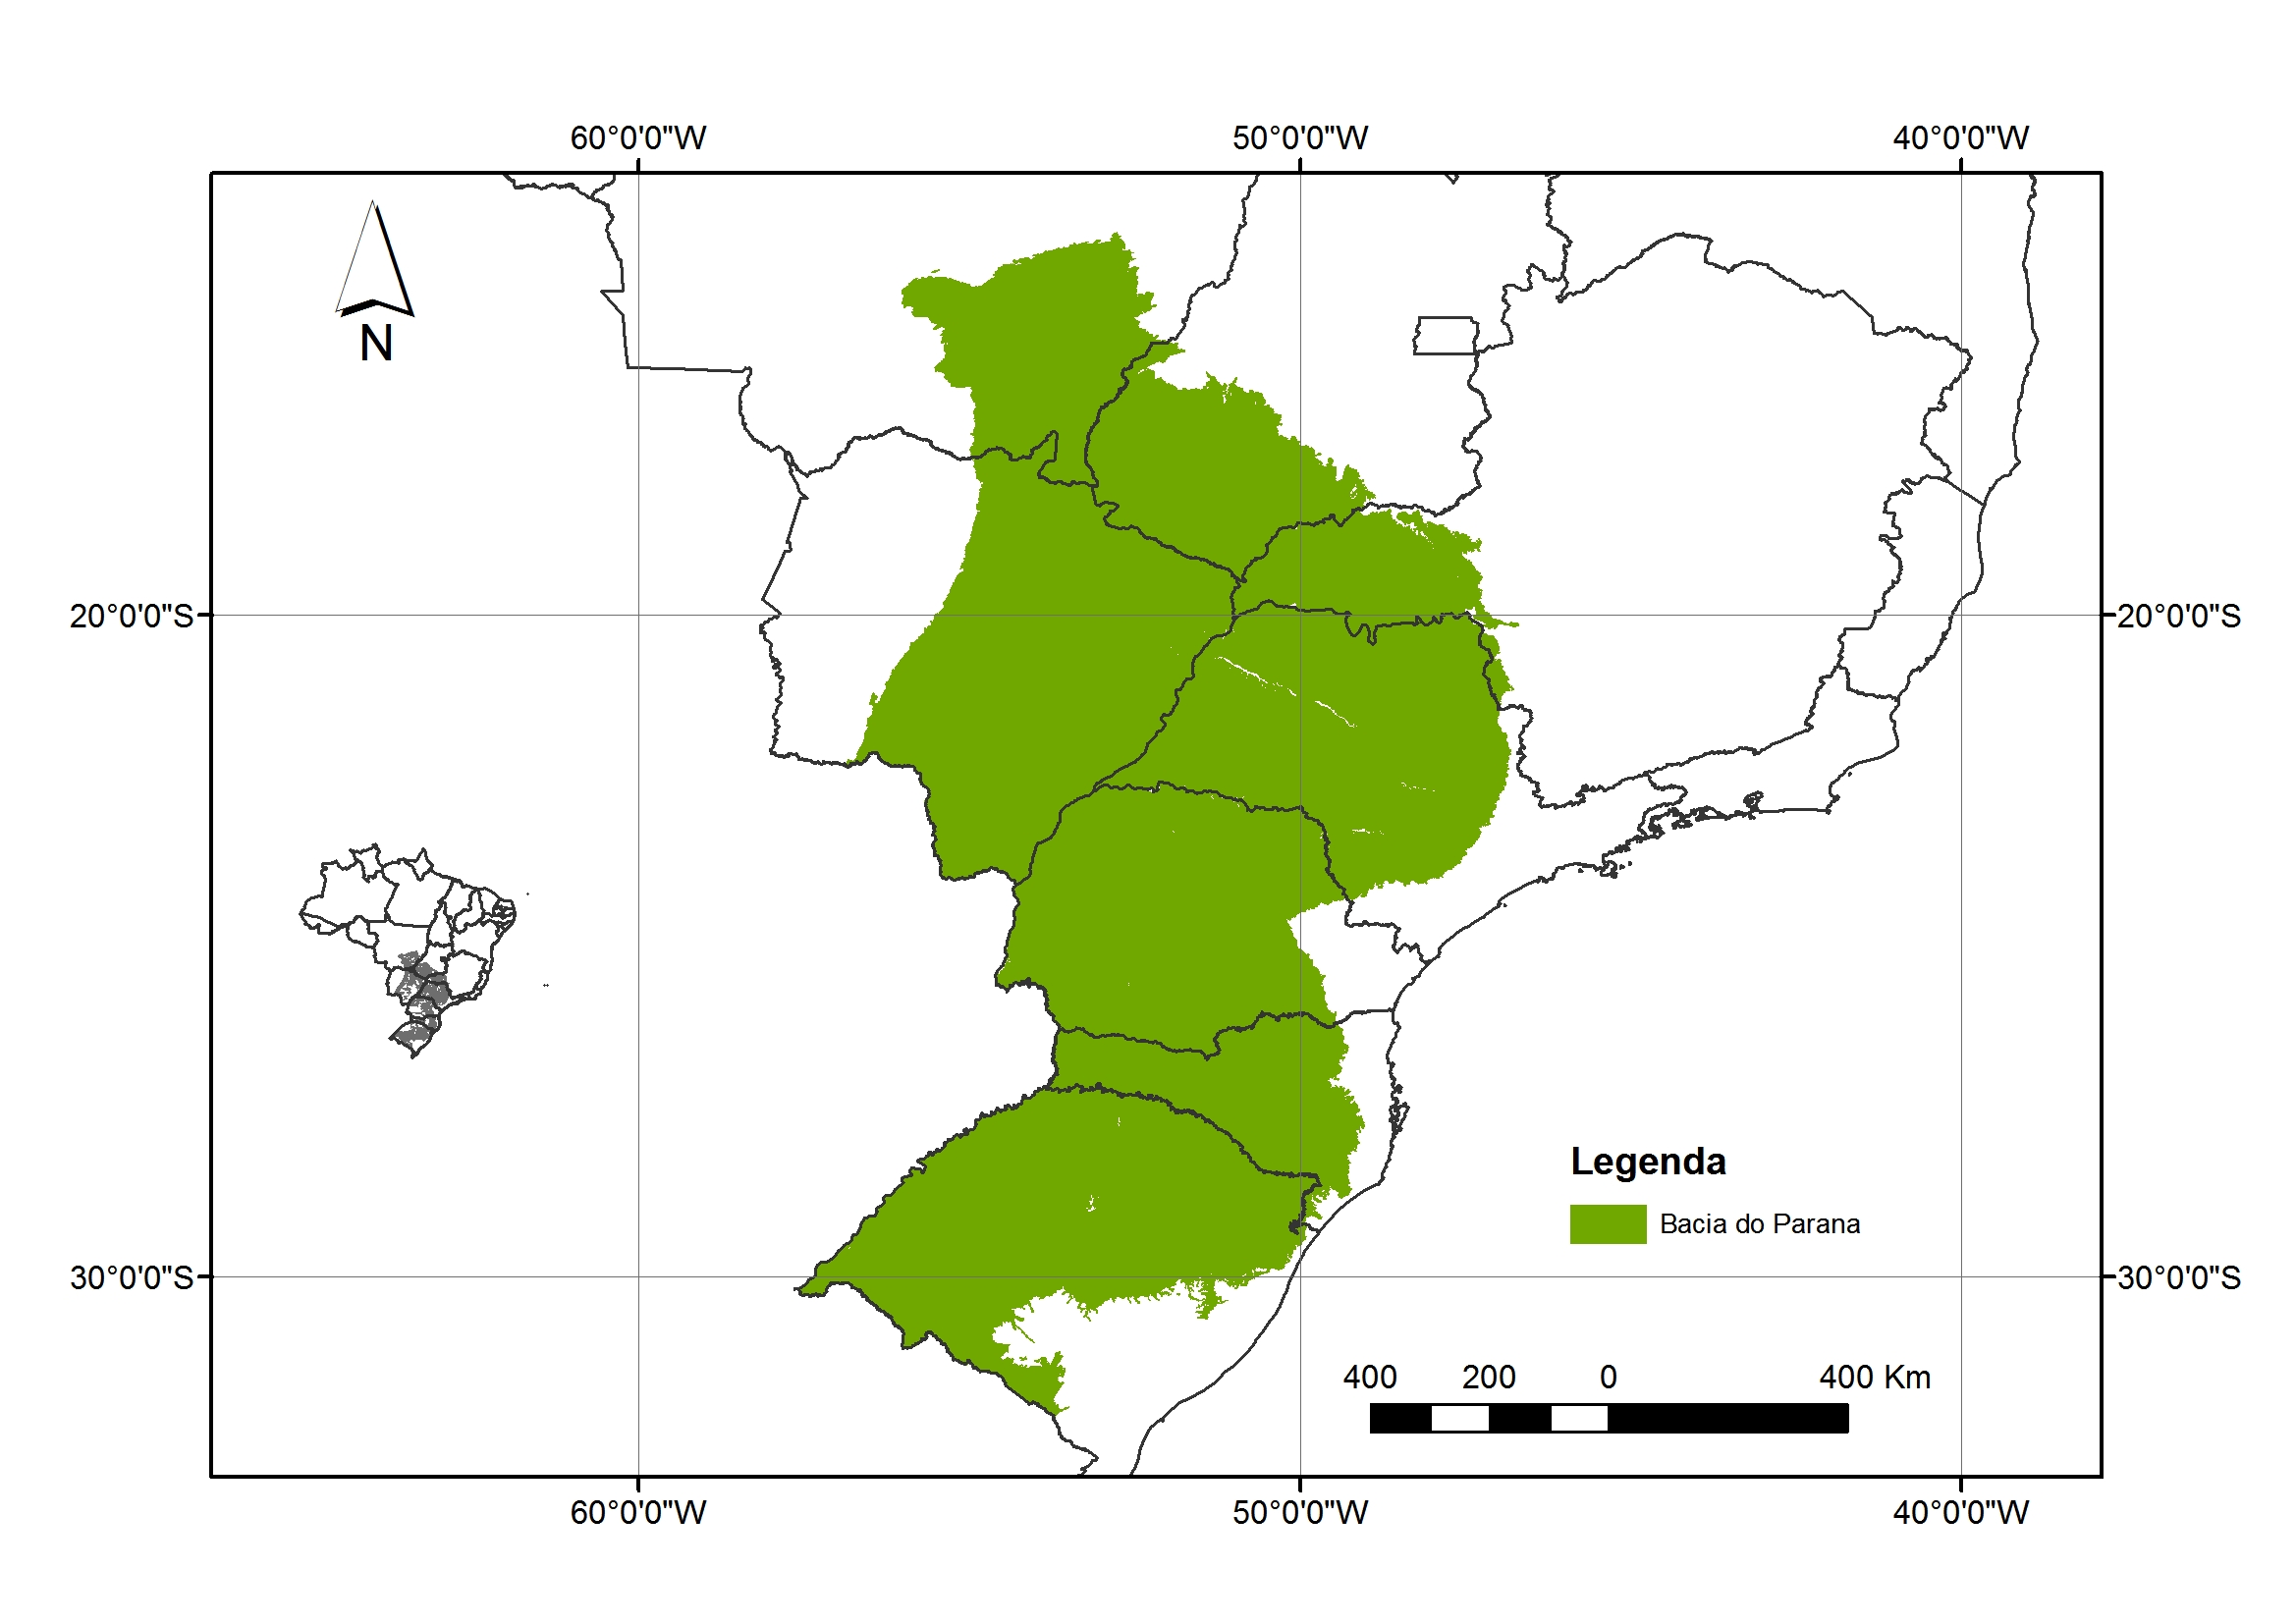
\includegraphics[scale=0.4]{Imagens/BaciaParana.jpg}
	}
	\caption{Mapa geológico e de localização da área de estudo. }
	\label{mapa geologico}
\end{figure}


  \chapter{Método Proposto e Objetivo}

A parte operacional deste programa se divide em duas etapas: 1- Geração de dados sintéticos, 2- Treinamento e 3- Identificação. Cada uma destas etapas será realizada por um programa computacional específico, este programas vão funcionar de forma independente.

O primeiro programa tem por objetivo gerar dados sintéticos que devem simular os resultados obtidos num levantamento de um perfil composto.

O programa da etapa de Treinamento será alimentado com dados de perfilagens cujas respectivas fácies litológicas são conhecidas (inicialmente serão usados dados sintéticos e posteriormente dados reais). Este programa vai gerar um arquivo com os dados do treinamento, este arquivo será usado pelo programa de Operação. Esta é a fase de aprendizagem da rede.

O programa da etapa de identificação vai fazer a classificação, de forma autônoma, das facies litológicas em poços a partir de dados de perfilagem em poços nos quais a litologia é desconhecida. A aprendizagem da rede deve ocorrer de forma continuada, quanto mais informação temos sobre situações nas quais a litologia é conhecida mais bem preparada estará a rede em termos de aprendizagem. Este conceito de aprendizagem é acumulativo e isso ocorrerá através da atualização do arquivo com os dados de treinamento.

Durante a elaboração dos programas será necessário testar a usa eficiência. Estes testes serão realizados através de dados sintéticos que serão gerados por um terceiro programa, gerador de dados sintéticos. Este programa será alimentados com informações da literatura. Após os testes com dados sintéticos a metodologia será validada com dados reais, posteriormente depois de cumpridas todas estas etapas, a metodologia estará pronta para ser utilizada em situações reais.

É importante salientar que neste método o conhecimento do funcional geofísico que rege a relação entre a litologia e a propriedades físicas das rochas não é necessário durante o processo. O conceito de inteligência artificial que será utilizado prescinde do funcional geofísico, o aprendizado é feito através da identificação de padrões recorrentes.

O ponto positivo desta metodologia é prescindir do funcional geofísico, que por vezes é desconhecido ou de alta complexidade o que exige uma modelagem matemática trabalhosa.

O ponto negativo é a necessidade de se ter muitos dados já analisados em situações conhecidas e variadas para a realização da etapa de treinamento. A etapa de treinamento tem um custo computacional alto.

\section{Objetivo}
O principal objetivo deste projeto é desenvolver um programa computacional do tipo “ machine learning ”, que será implementado na forma de uma Rede Neural Artificial (RNA) dentro do contexto da inteligência artificial. Este programa deve ter a capacidade de identificar, de forma autônoma, fácies litológicas a partir de dados de perfilagem de poços sem a necessidade do uso de um funcional geofísico.

É importante salientar que a metodologia que será desenvolvida neste projeto tem aplicação direta tanto na indústria de exploração mineral, quanto na de água, e na de petróleo e gás.

  \chapter{Dados de Perfilagem}

As RNAs são capazes de reconhecer padrões \citep{Konate2014,Kumar2015}. E padrões muitas vezes são recorrentes no tocante a geologia \citep{Vail_1977}. 

Ciclos de deposição de siltes e argilas e areias muitas vezes são controlados pelas variações constantes das estações do ano \citep{Milani1998,CristinaLopesQuintas1999,Milani2000} . Esse registro litológico se faz presente em dados de poços em todo o mundo \citep{Scherer2006}.

Em uma perfilagem de poço composta são realizadas diversas medidas de propriedades físicas que ao serem analisadas, em conjunto, tornam possível ao geólogo identificar mudanças litológicas e consequentemente topos e bases de camadas de interesse \citep{FrancaAlmerio&Potter1991,Zalan2007,artur_paleoestruturas_2008}. 

A Fig. \ref{PerfilComposto} ilustra a disposição de um perfil de poço associado com topos e bases de rochas. 

\begin{figure}[H]
		\centering
	\setlength{\fboxsep}{8pt}
	\setlength{\fboxrule}{0.1pt}
	\fbox{
	\includegraphics[scale=0.16]{Imagens/poco.png}
}
	\caption{Exemplo de um dado público de uma perfilagem de poço composta realizada pela Petrobras, na Bacia do Paraná.}
	\label{PerfilComposto}
\end{figure}

Entretanto não é toda a perfilagem de poço que contém o topo e base de camada. As RNAs se apresentam como uma solução para o problema de identificação litológica e dos topos e bases dessas camadas. Uma vez observado que a variação das propriedades físicas das rochas em subsuperfície variam obedecendo certos padrões \citep{Yan2014}. 

Em \citet{Telford_1993}, encontram-se variações das propriedades físicas dos principais grupos de rochas. A Tab. \ref{rock-properties1} e a Tab. \ref{rock-properties2} apresentam um compêndio desses principais valores.  

\begin{table}[H]
	\centering
	\caption{Compilação de Perfis usados na inferência de litologia.}
	\label{rock-properties1}
	\begin{tabular}{@{}llllllllll@{}}
		\toprule
		Rocha         & Densidade ($g/cm^{3}$) & Raios-Gama ($Ci/g$)& Potencial-Espontâneo ($mV$)&   \\ \midrule
		Conglomerado &     $2,50$  &       ---        &    ---        &      \\
		Arenito  &    $2,35$      &       $2,00\leftrightarrow4,00$       &     ---       &      \\
		Folhelho &   $2,40$       &      ---        &      ---      &    \\
		Argilito &     $2,55$   &          ---     &       ---     &     \\
		Siltito  &      $2,21$    &          ---     &       ---     &   \\
		Dolomita &     $2,70$    &        $8,00$       &   ---         &       \\
		Marga  &    $2,50$     &         ---      &    ---        &     \\
		Basalto  &     $2,99$    &          $0,50$     &    ---       &      \\
		Diabásio &    $2,90$    &         ---      &       ---     &     \\
		Lava &     $2,61$    &      $0,33$         &      ---      &      \\
		Granito &    $2,64$      &       $0,70\leftrightarrow4,80$        &      ---      &      \\
		Gabro &    $3,03$     &       ---        &     ---       &       \\
		Peridotito &   $3,15$    &      ---         &     ---       &      \\
		Quartzito &    $2,60$    &        $5,00$      &     ---       &    \\
		Xisto &   $2,64$    &         ---      &      ---      &    \\
		Gnaisse &    $2,80$     &      ---         &    ---        &        \\
		Serpentinito &    $2,78$     &   ---            &   ---     &        \\
		Anfibolito &  $2,96$       &          ---     &       ---     &        \\
		Eclogito &  $3,37$    &       ---        &      ---      &    \\
		Mármore &   $2,75$       &      ---         &     ---       &      \\ \bottomrule
	\end{tabular}
\end{table}

\begin{table}[H]
	\centering
	\caption{Compilação de Perfis usados na inferência de porosidade, permeabilidade.}
	\label{rock-properties2}
	\begin{tabular}{@{}llllllllll@{}}
		\toprule
		Rocha   & Resistividade ($\Omega/m$) &  Neutrão ($API$) & Velocidade ($km/s$)  &    \\ \midrule
		Conglomerado &    $2\times10^{3}\leftrightarrow10^{4}$       &    ---           &     $1,80\leftrightarrow4,90$       &     \\
		Arenito  &    $1\leftrightarrow6,4\times10^{8}$       &      ---         &     $4,00\leftrightarrow4,30$       &   \\
		Folhelho &     $50\leftrightarrow10^{7}$      &      ---         &      $2,15\leftrightarrow3,30$      &   \\
		Argilito &     $10\leftrightarrow8\times10^{2}$      &       ---        &     ---       &      \\
		Siltito  &      $1\leftrightarrow100$     &      ---         &         $4,00\leftrightarrow6,20$    &         \\
		Dolomita &   $3,5\times10^{2}\leftrightarrow5\times10^{3}$        &    ---           &      $5,70\leftrightarrow6,00$      &      \\
		Marga  &     $3\leftrightarrow70$      &     ---          &     ---       &     \\
		Basalto  &     $10\leftrightarrow1,3\times10^{7}$      &     ---          &     $ 5,00\leftrightarrow5.80$         &     \\
		Diabásio &  $20\leftrightarrow5\times10^{7}$         &      ---         &     ---       &  \\
		Granito Porfirítico (seco) &     $1,3\times10^{6}$     &       ---        &     $5,80$       &    \\
		Granito Porfirítico (úmido) &  $4,5\times10^{3}$          &      ---         &     $ 5,00\leftrightarrow5.60$         &      \\
		Gabro &   $10^{3}\leftrightarrow10^{6}$       &      ---         &      $ 5,00\leftrightarrow5.80$        &     \\
		Peridotito (seco) &   $6,5\times10^{3}$        &    ---           &       ---     &    \\
		Peridotito (úmido) &    $3\times10^{3}$       &      ---         &      ---      &  \\
		Xisto &    $20\leftrightarrow10^{4}$       &        ---       &       ---     &   \\
		Gnaisse (seco) & $3\times10^{6}$          &         ---      &     ---       &   \\
		Gnaisse (úmido) &   $6,8\times10^{4}$        &       ---        &      ---      &   \\
		Tufa (seca) &      $2\times10^{3}$     &      ---         &     $1,80\leftrightarrow3,50$       &     \\
		Tufa (úmida) &     $10^{5}$      &     ---          &     ---       &      \\
		Mármore &  $10^{2}\leftrightarrow2,5\times10^{8}$         &       ---        &      ---      &    \\ \bottomrule
	\end{tabular}
\end{table}

%FALAR DO TRATAMENTO DO DADO, DO NEURÔNIO, DA GEOMETRIA DA REDE, DO TREINO, DA FUNÇÃO DE ATIVAÇÃO, CAMADAS OCULTAS, PESOS.%
 

\section{Modelo proposto para gerar os dados sintéticos}

O modelo proposto para o teste da rede neuronal foi concebido com base em um modelo geológico esquemático proposto por  \citet{Sal2008} \textit{apud} \citep{Eiras1996}. Esta simplificação reproduz, em uma bacia do tipo sinéclise, estruturas geológicas como Horts, Grábens, semi-grábens, falhas normais, reversas. E representa ainda processos halocinéticos referenciados por \cite{Eiras1996}.

A Fig. \ref{modelo} representa o modelo em tratado anteriormente. A caixa aumentativa evidencia a falha normal, representada no dado de poço por um contato não plano-paralelo.

\begin{figure}[H]
	\centering
	\setlength{\fboxsep}{8pt}
	\setlength{\fboxrule}{0.1pt}
	\fbox{
		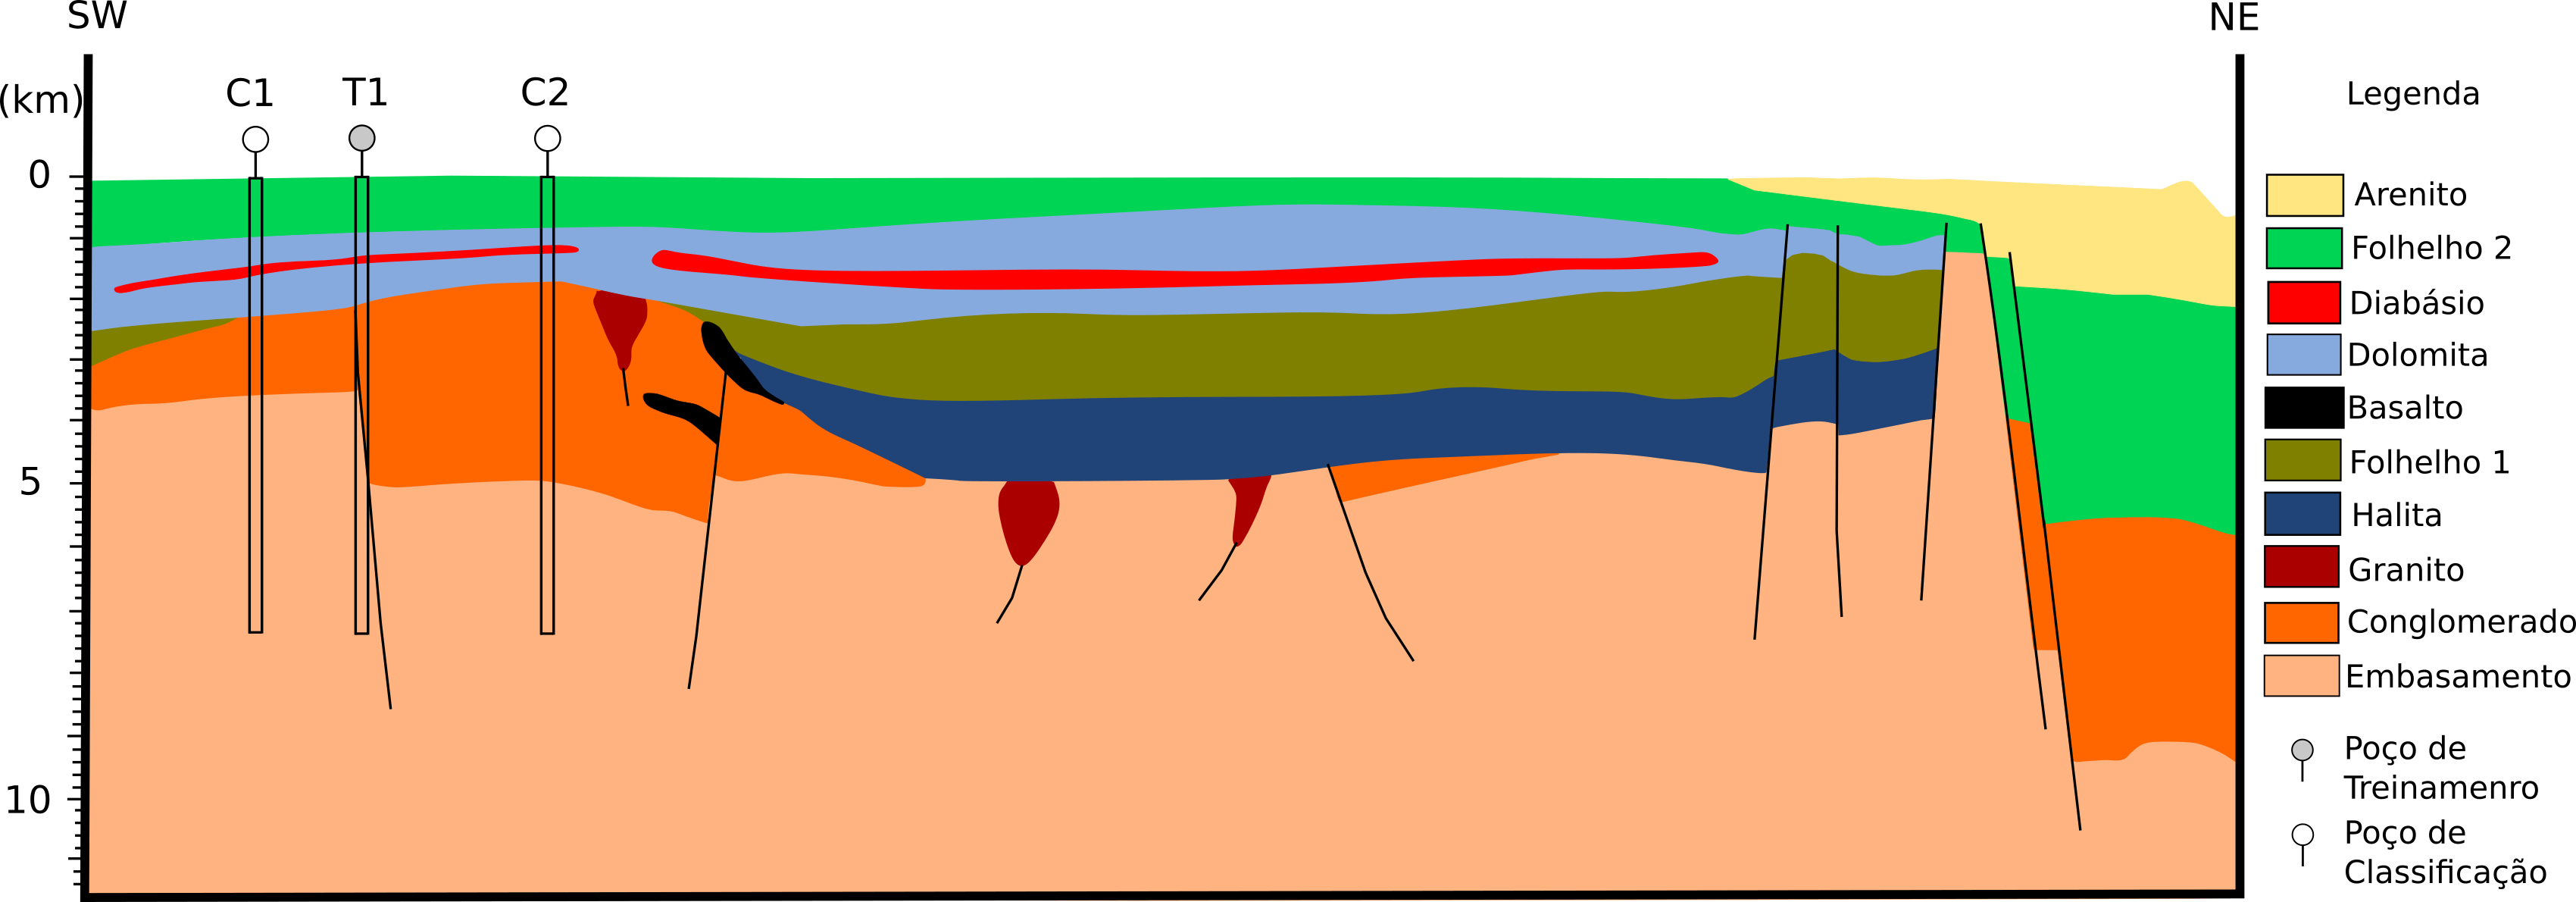
\includegraphics[scale=0.5]{Imagens/Modelo.png}
	}
	\caption{Modelo Simplificado baseado em \cite{Sal2008}.}
	\label{modelo}
\end{figure}

A partir da Fig. \ref{modelo} foram gerados três poços, na parte SW do perfil, com profundidades de $7$ km cada. Os três poços contém um conjunto com $4$ dados de propriedades físicas que são densidade, raio-gama, resistividade e velocidade, respectivamente. Os valores de propriedades físicas utilizados foram  baseados, em resultados já publicados, na literatura geocientífica, anteriormente, e retirados de \citet{Telford_1993}. Os poços simulam dados de \textit{well logging} com uma taxa de amostragem de $10$ m.

Os poços simulam diferentes padrões interpretativos usuais da ciência de perfilagem \footnote{Padrões usuais reconhecido por intérpretes geralmente associados a horizontes de interesse. Esses padrões são identificados como padrões sinos, sinos invertidos, serra e caixa.}. O poço denominado T$1$ \footnote{T$1$: poço escolhido para treinar a rede neuronal.} se localiza entre os poços C$1$ e C$2$ atravessando uma falha normal. 

A Fig. \ref{T1} apresenta os dados do poço T1. As espessuras das camadas são de $800$ m de embasamento, $2$ km de uma mistura crescente entre conglomerado e embasamento, perfazendo um padrão sino nos dados de perfilagem, $2$ km de conglomerado, $1$ km de dolomita (pacote inferior), $300$ m de diabásio, $400$ m de dolomita (pacote superior), $600$ m de folhelho $2$. A falha foi representada por uma função linear da variação de profundidade por propriedade física de uma mistura crescente de conglomerado e embasamento.

\begin{figure}[H]
	\centering
	\setlength{\fboxsep}{8pt}
	\setlength{\fboxrule}{0.1pt}
	\fbox{
		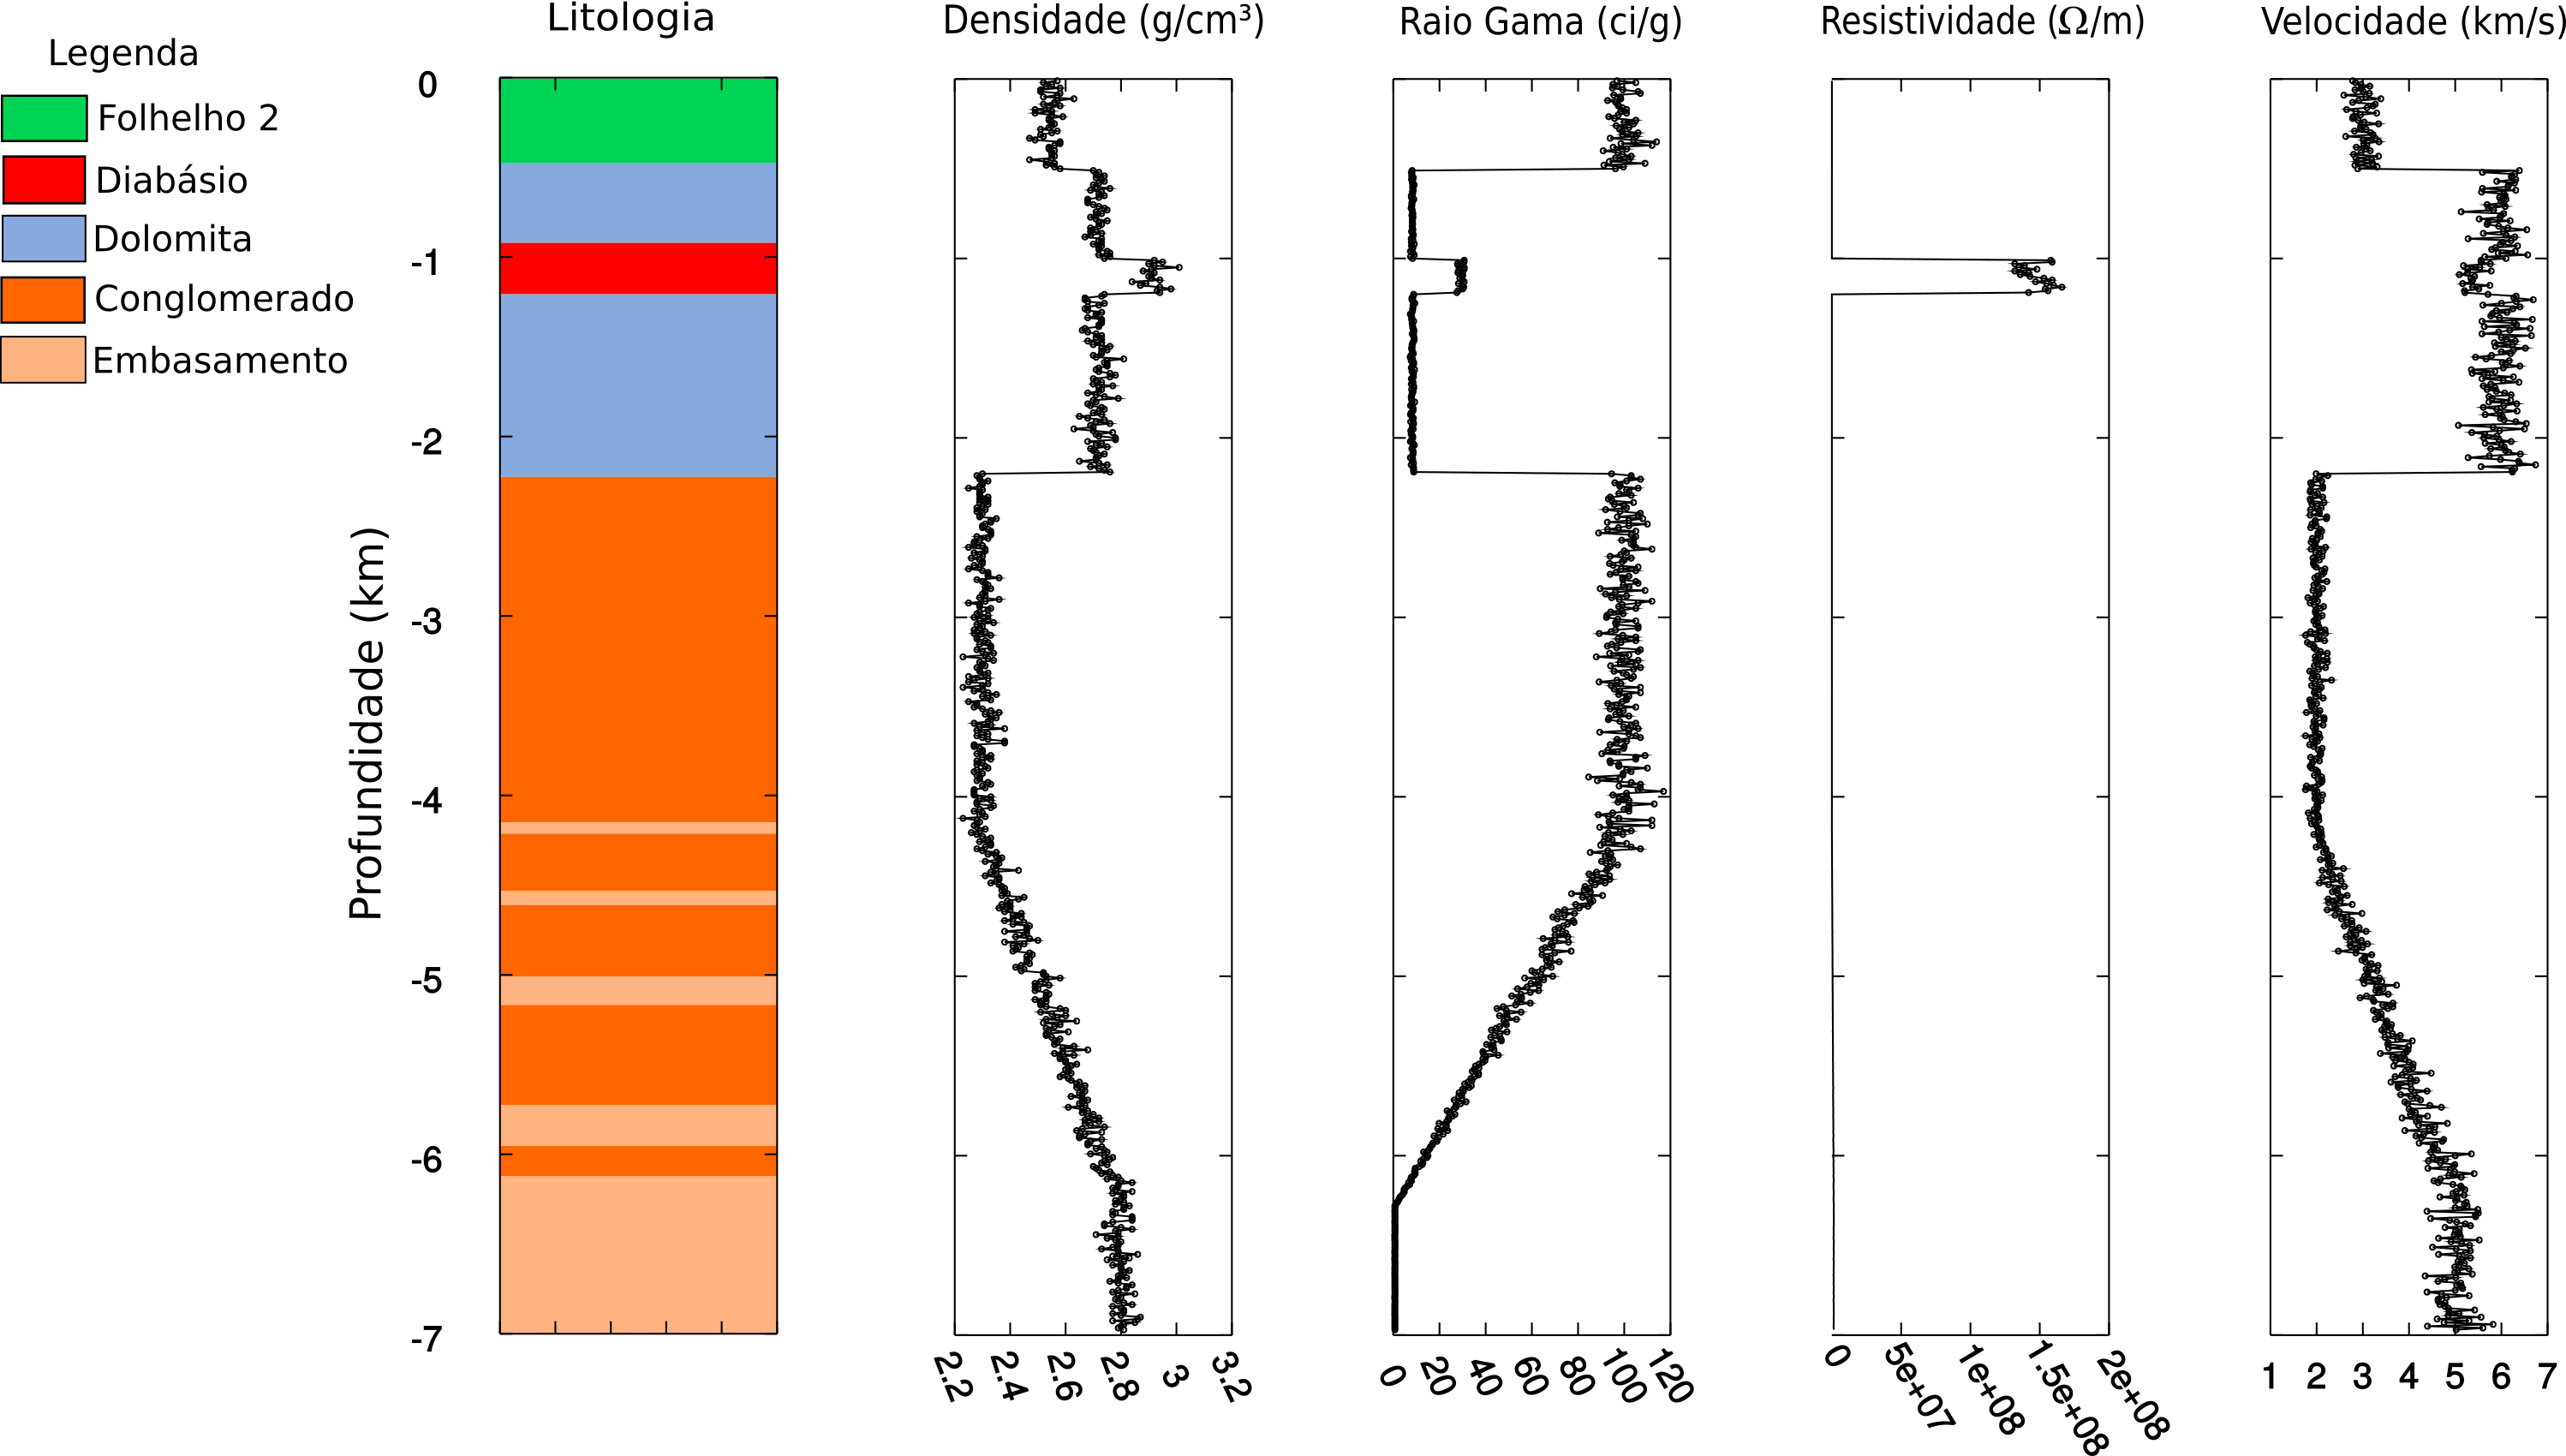
\includegraphics[scale=0.5]{Imagens/PocoT1.png}
	}
	\caption{Dado de perfilagem sintético, T1. Aonde a porcentagem de CE indica a mistura de conglomerado com embasamento}
	\label{T1}
\end{figure}

O poço C$1$\footnote{C1: Poço de classificação da rede neuronal número 1.}, Fig. \ref{C1}, possui as mesmas classes de rochas do poço T$1$. A escolha da posição dos poços quase que exclusivamente na parte SW do perfil se deu em virtude da localização do poço T$1$. Uma vez que espera-se da rede já treinada um reconhecimento das classes já estudadas. Os pacotes sedimentares apresentam espessuras de $2,8$ km de embasamento, $1,6$ km de conglomerado, $1$ km de dolomita (segundo pacote), $200$ m de diabásio, $500$ m de dolomita (primeiro pacote) e $500$ m de folhelho. 

\begin{figure}[H]
	\centering
	\setlength{\fboxsep}{8pt}
	\setlength{\fboxrule}{0.1pt}
	\fbox{
		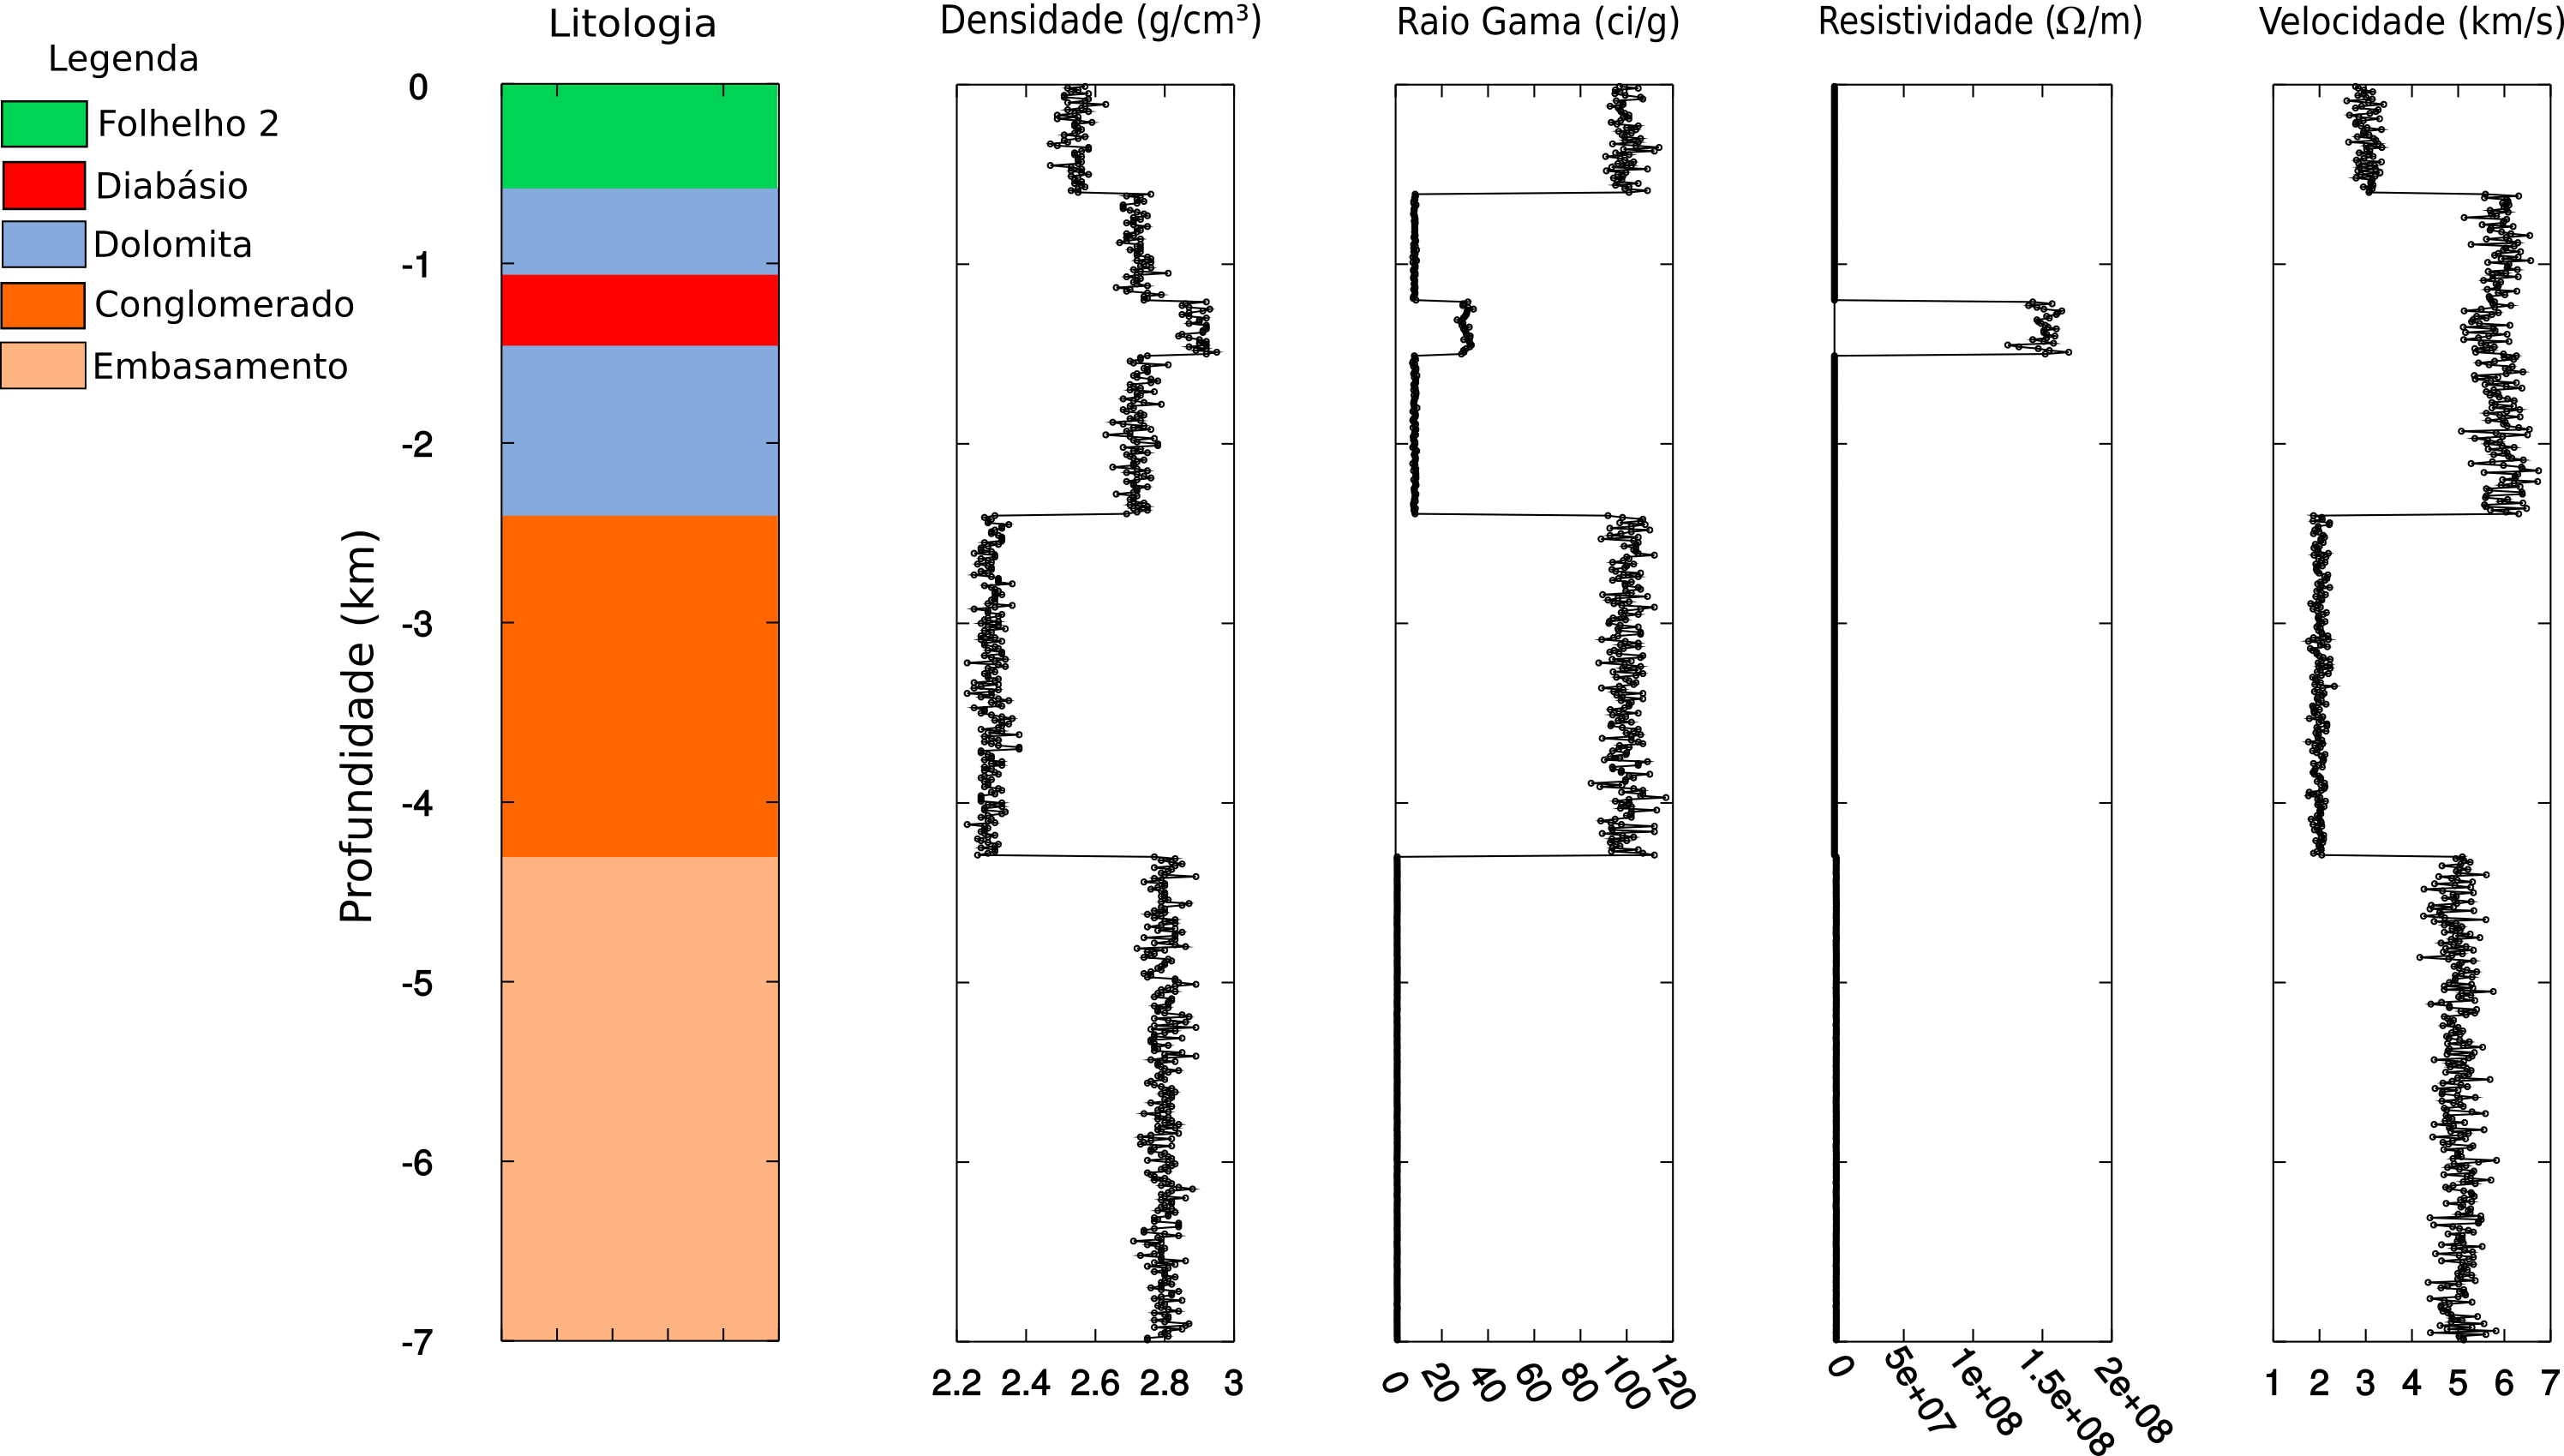
\includegraphics[scale=0.5]{Imagens/PocoC1.png}
	}
	\caption{Dado de perfilagem sintético, C1.}
	\label{C1}
\end{figure}

O poço C$2$\footnote{C2: Poço de classificação da rede neuronal número 2.}, Fig. \ref{C2}, localiza-se em um alto estrutural, e apresenta espessura de $5$ km de conglomerado. O embasamento possui uma espessura de $1,8$ km. Os pacotes de folhelho 2, dolomita (pacote superior) e diabásio $500$ m respectivamente. E o segundo pacote sedimentar de dolomita $1,6$ km.

\begin{figure}[H]
	\centering
	\setlength{\fboxsep}{8pt}
	\setlength{\fboxrule}{0.1pt}
	\fbox{
		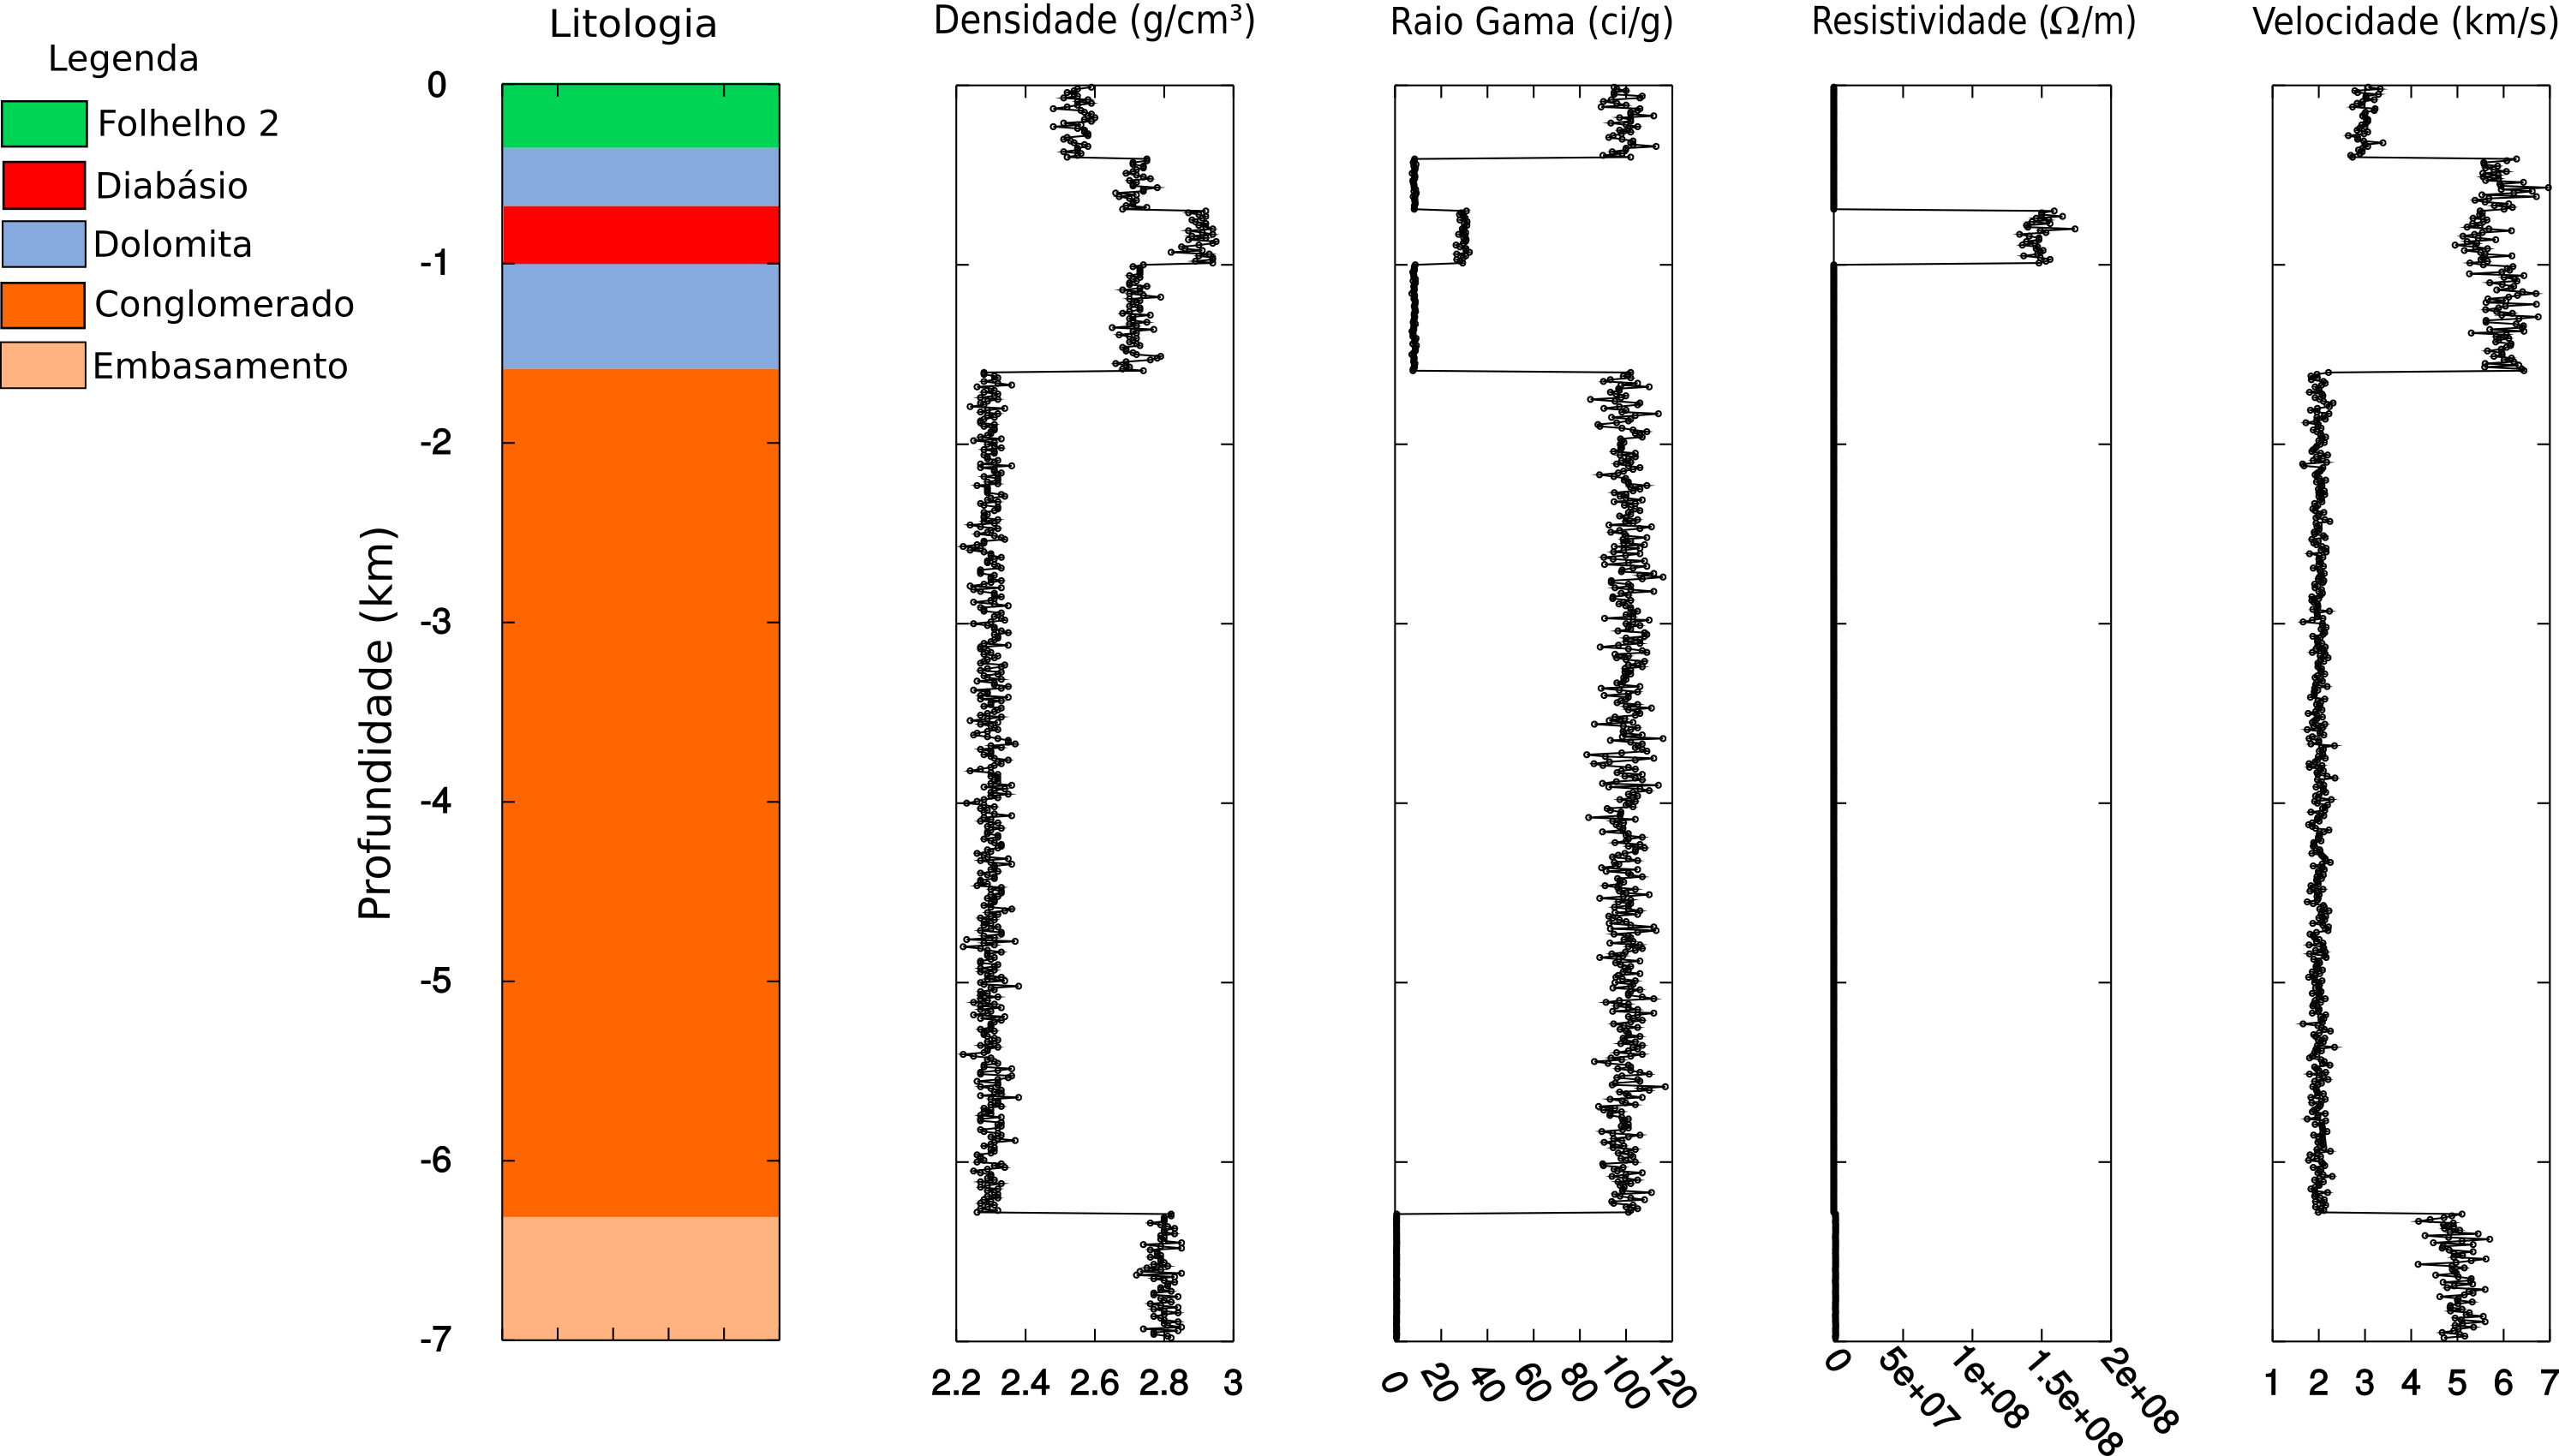
\includegraphics[scale=0.5]{Imagens/PocoC2.png}
	}
	\caption{Dado de perfilagem sintético, C2.}
	\label{C2}
\end{figure}

\section{Dado Real}

A triagem dos dados públicos contemplaram  $506$ arquivos *.dlis, $113$ *.lis, $118$ dados adicionais, $125$ perfis compostos digitalizados, $174$ poços públicos, $120$ arquivos *.agp, todos localizados na Bacia Sedimentar do Paraná. 

O conjunto de dados *.lis e *.dlis estão sendo convertidos para arquivos em formato texto, que serão posteriormente concatenados  com os arquivos *.agp afim de se obter o input da rede. Este processo ainda se encontra na fase inicial com cerca de $3\%$ concluído.

A Fig. \ref{real} mostra a localização e distribuição dos poços na Bacia do Paraná.

\begin{figure}[H]
	\centering
	\setlength{\fboxsep}{8pt}
	\setlength{\fboxrule}{0.1pt}
	\fbox{
		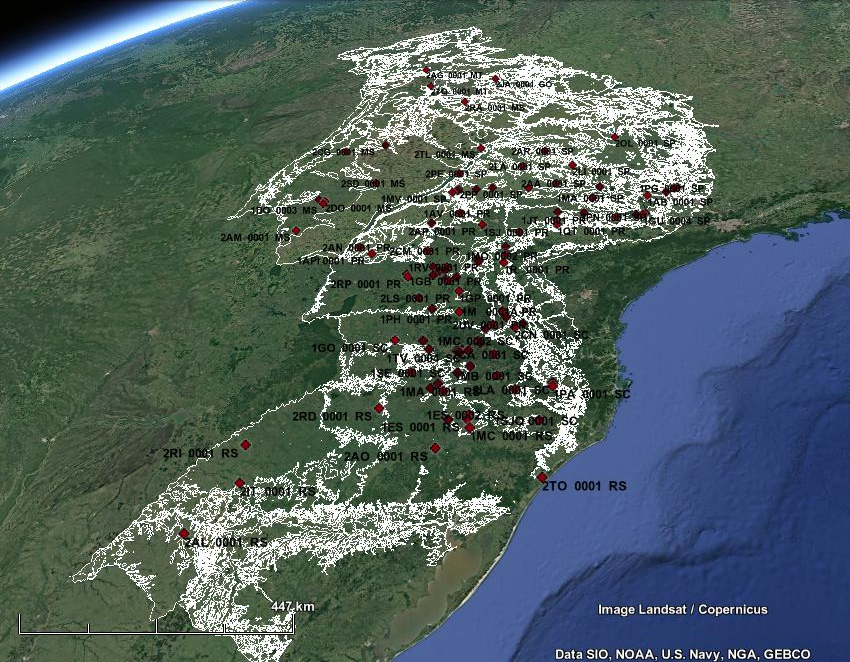
\includegraphics[scale=0.5]{Imagens/Pocos.jpg}
	}
	\caption{Localização dos poços de trabalho.}
	\label{real}
\end{figure}



  \chapter{Resultados e Discussões}

A Fig. \ref{clusterT1} apresenta à variação das propriedades físicas analisadas por agrupamento de classes de rochas para o poço T$1$. 

\begin{figure}[H]
	\centering
	\setlength{\fboxsep}{8pt}
	\setlength{\fboxrule}{0.1pt}
	\fbox{
		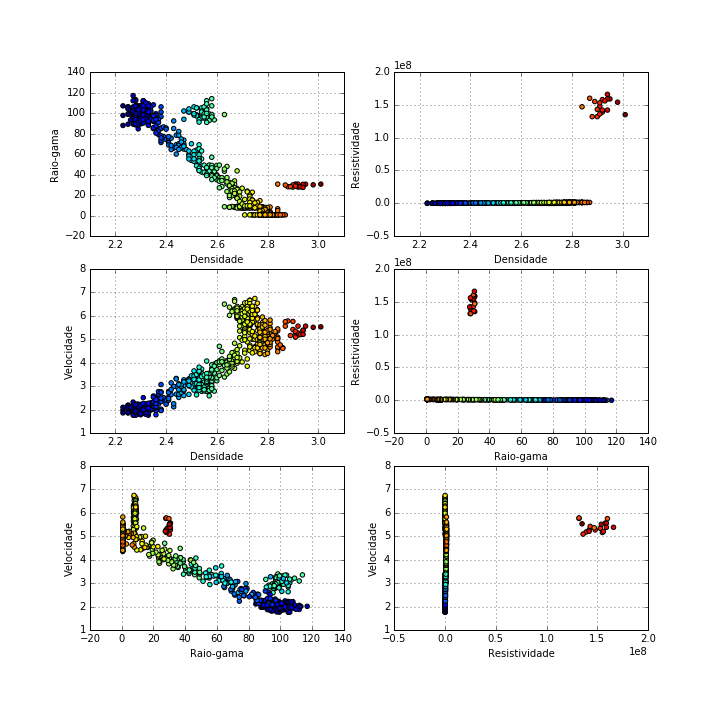
\includegraphics[scale=0.5]{Imagens/cluterpocoT1.png}
	}
	\caption{Agrupamento de dados do poço T1.}
	\label{clusterT1}
\end{figure} 

É perceptível o notável contraste de variação das propriedades físicas entre a rocha de origem ígnea, em contraste com as propriedades físicas das demais rochas de origem sedimentar e metamórfica. 

A Fig. \ref{clusterC1} apresenta à variação das propriedades físicas analisadas por agrupamento de classes de rochas para o poço C$1$. Em destaque, de vermelho, o litotipo diabásio. 

\begin{figure}[H]
	\centering
	\setlength{\fboxsep}{8pt}
	\setlength{\fboxrule}{0.1pt}
	\fbox{
		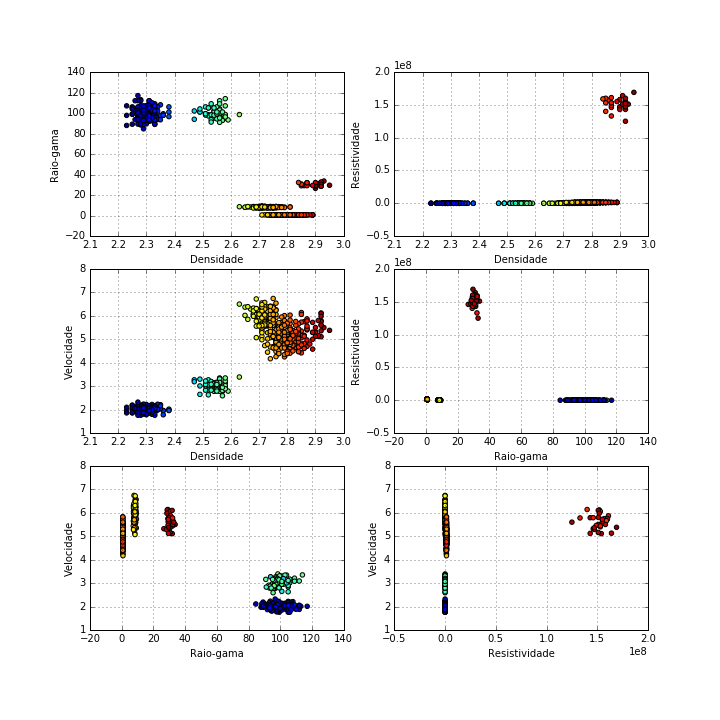
\includegraphics[scale=0.5]{Imagens/cluterpocoC1.png}
	}
	\caption{Agrupamento de dados do poço C1.}
	\label{clusterC1}
\end{figure} 

Neste caso, o agrupamento das classes de rochas é mais evidente, no gráfico de raio-gama por densidade, que evidencia os $5$ litotipos distintamente. E, da mesma maneira, o gráfico de velocidade por densidade.


A Fig. \ref{clusterC2} apresenta à variação das propriedades físicas analisadas por agrupamento de classes de rochas para o poço C$2$. Em destaque, de vermelho, o litotipo diabásio. 

\begin{figure}[H]
	\centering
	\setlength{\fboxsep}{8pt}
	\setlength{\fboxrule}{0.1pt}
	\fbox{
		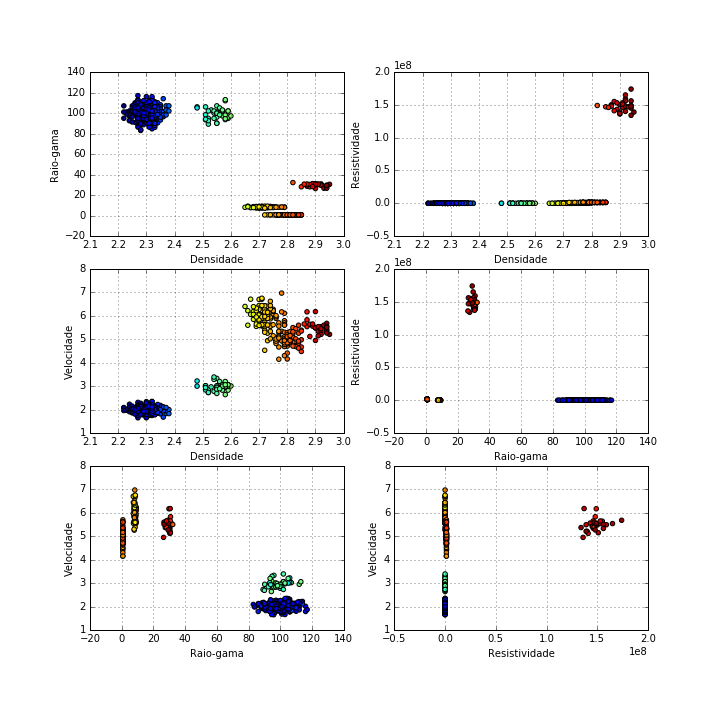
\includegraphics[scale=0.5]{Imagens/cluterpocoC2.png}
	}
	\caption{Agrupamento de dados do poço C2.}
	\label{clusterC2}
\end{figure} 

Na mesma forma, o agrupamento das classes de rochas é mais evidente, no gráfico de raio-gama por densidade, que evidencia os $5$ litotipos distintamente. E, da mesma maneira, o gráfico de velocidade por densidade.

\section{Treinamento}

A etapa de treinamento consiste em um ajuste de pesos dos neurônios da rede. Nesta fase, é identificado o neurônio que tem os valores dos pesos mais parecidos com os parâmetros de entrada da rede.  

\begin{figure}[H]
\centering
\subfigure[ref1][Iteração 1]{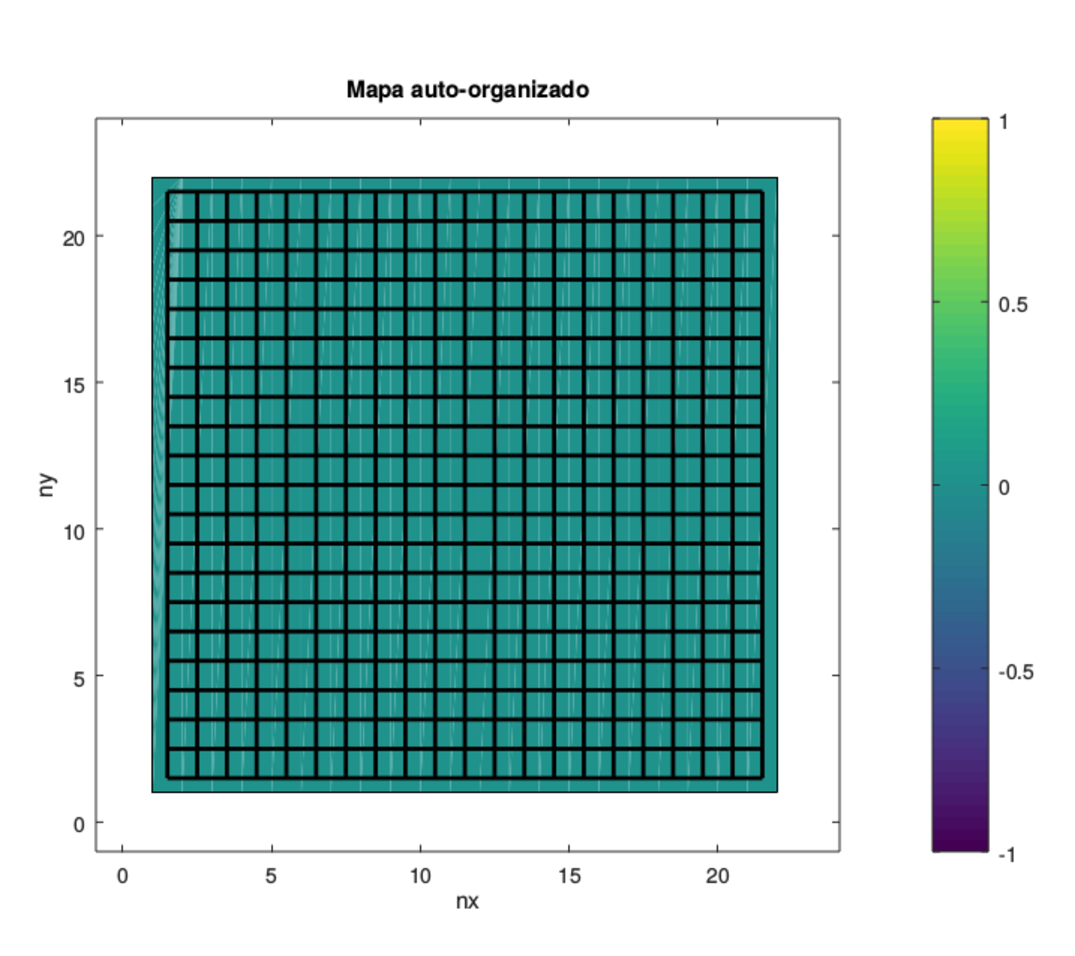
\includegraphics[width=7.0cm]{Imagens/SOM1_2d.pdf}}
\qquad
\subfigure[ref2][Iteração 5]{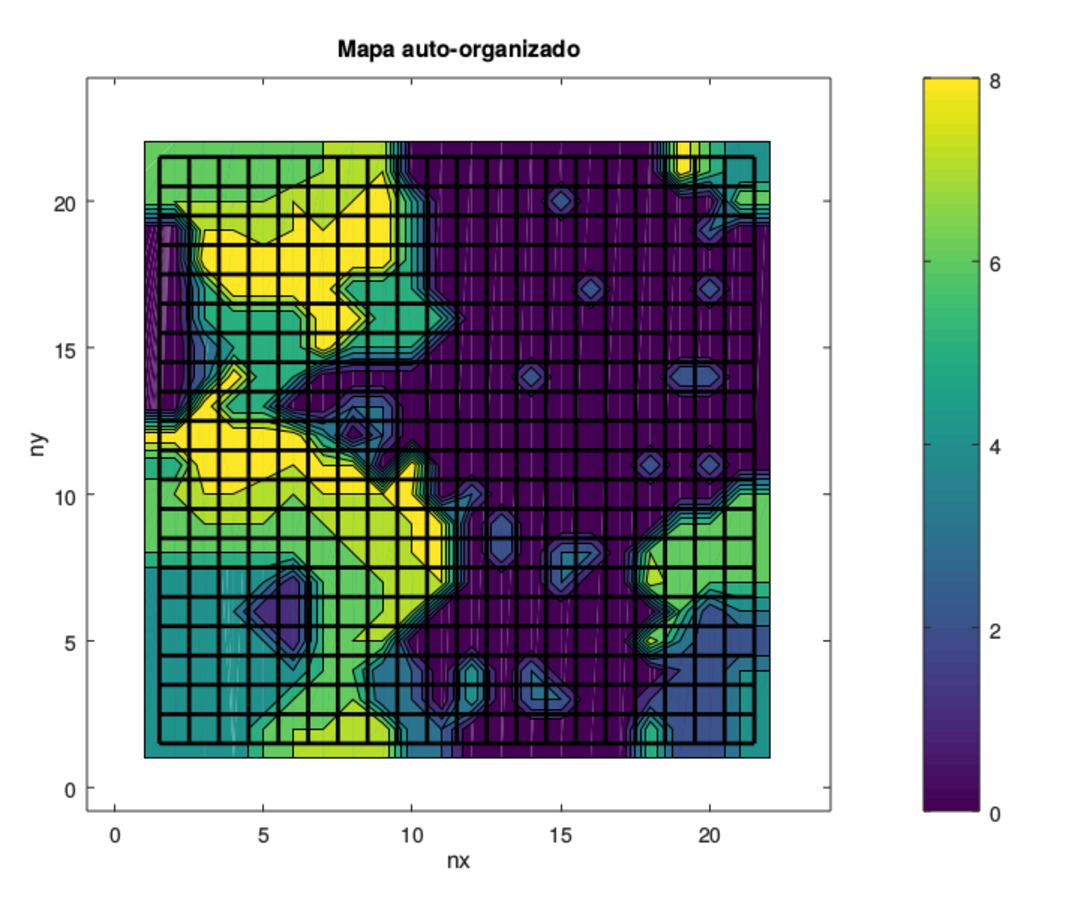
\includegraphics[width=7.0cm]{Imagens/SOM5_2d.pdf}}
\qquad
\subfigure[ref3][Iteração 100]{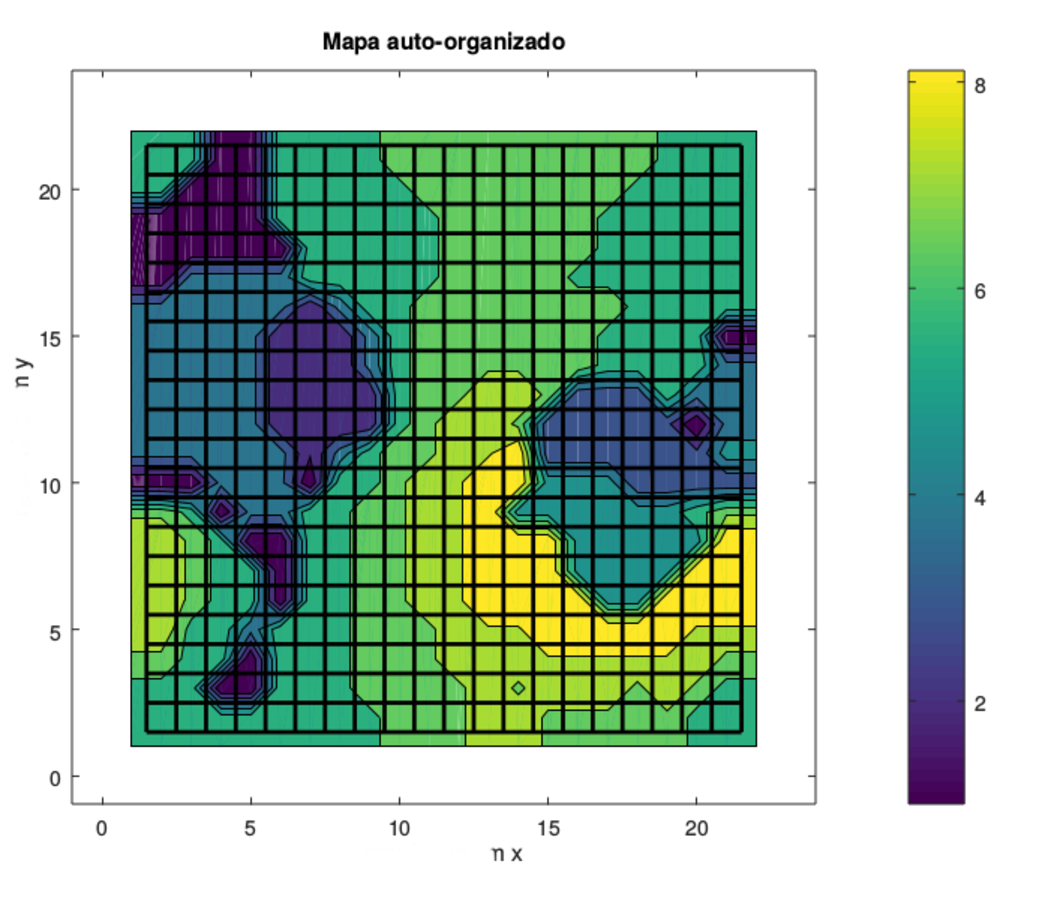
\includegraphics[width=7.0cm]{Imagens/SOM100_2d.pdf}}
\qquad
\subfigure[ref4][Iteração 1000]{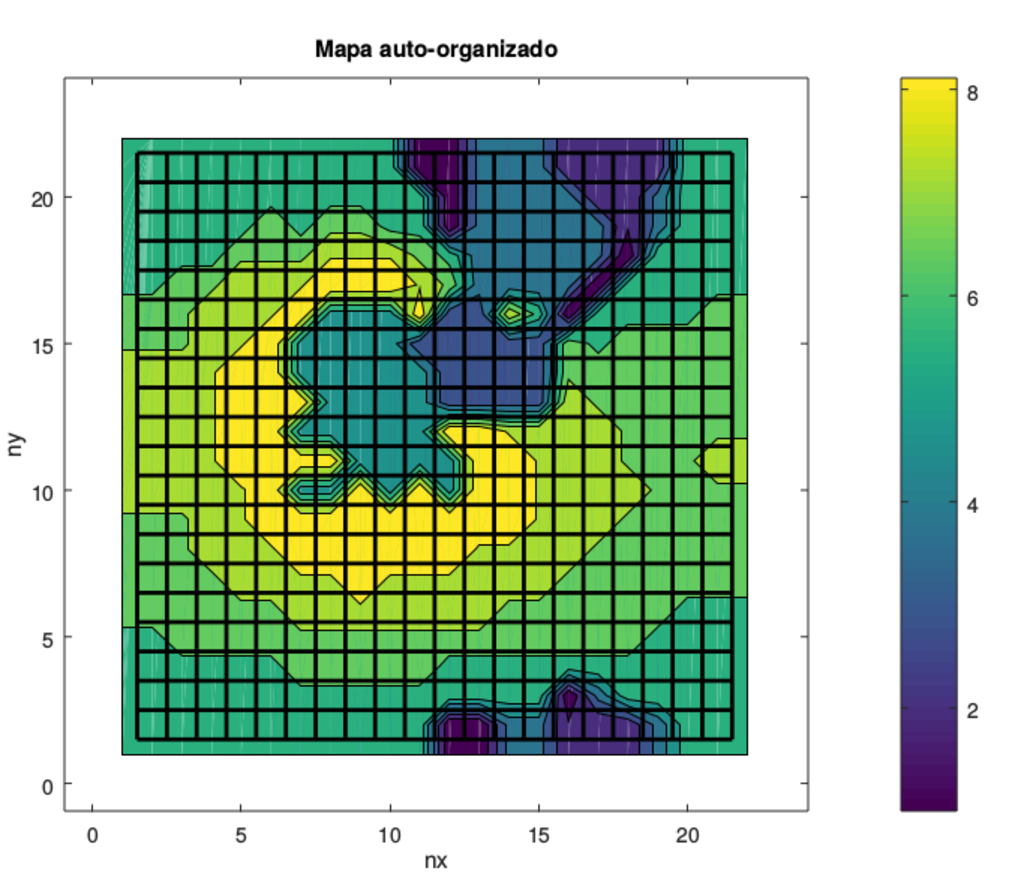
\includegraphics[width=7.0cm]{Imagens/SOM1000_2d.pdf}}
\qquad
\caption{Mapas auto-organizáveis e sua evolução temporal.}
\label{SOM}
\end{figure}

Os mapas da Fig. \ref{SOM} apresentam as zonas do hiperplano especializadas em identificar as classes de rochas. O código numérico $1$ representa folhelho, $2$ dolomita, $3$ diabásio, $4$ conglomerado, $5$ embasamento, $6$ mistura conglomerado/embasamento $75\%$, $7$ mistura conglomerado/embasamento $50\%$, $8$ mistura conglomerado/embasamento $25\%$.

A Fig. \ref{convergencia} apresenta o teste de convergência da rede neuronal.

\begin{figure}[H]
	\centering
	\setlength{\fboxsep}{8pt}
	\setlength{\fboxrule}{0.1pt}
	\fbox{
		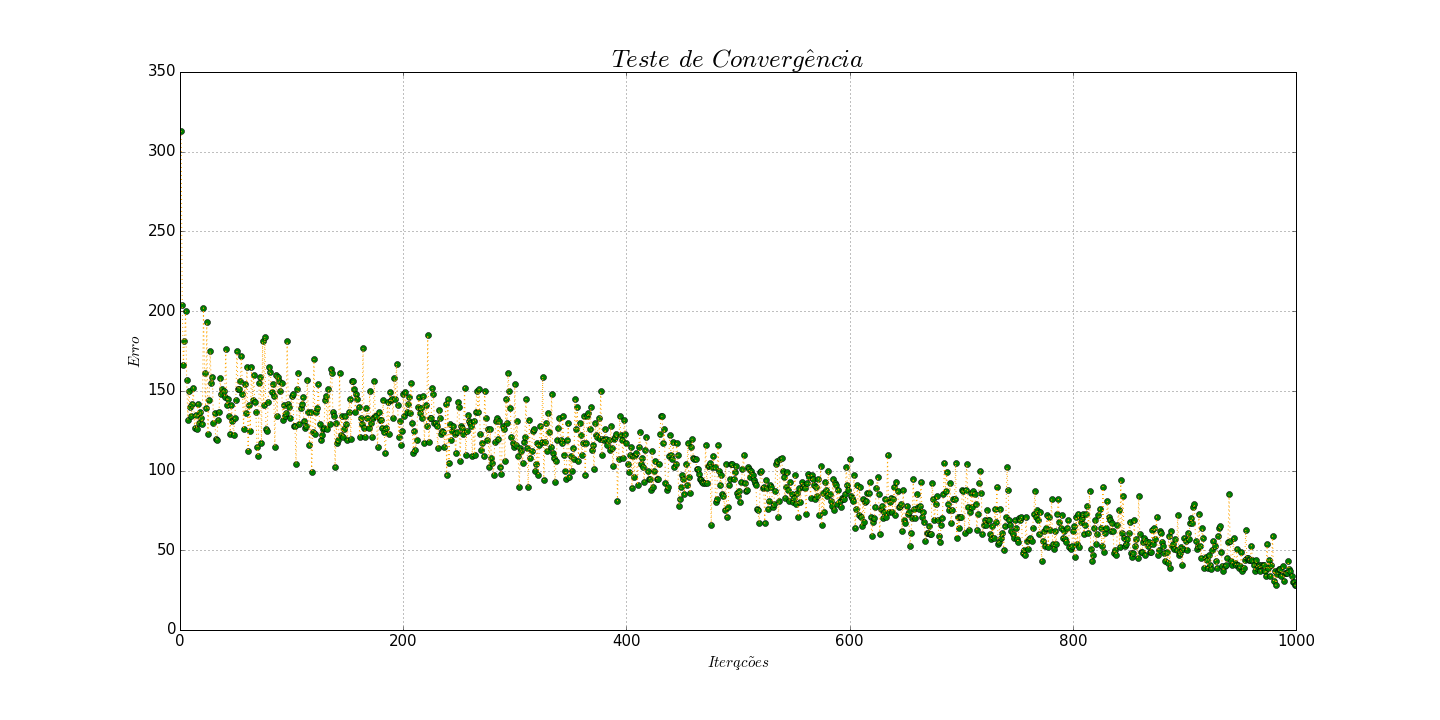
\includegraphics[scale=0.3]{Imagens/conv030917.png}
	}
	\caption{Teste de convergência da rede.}
	\label{convergencia}
\end{figure} 

O teste de convergência mostra que a rede se encontra estabilizada em  $1000$ iterações. Isto significa ser inócuo aumentar a iteração afim de diminuir o erro. 



\section{Identificação}




\begin{figure}[H]
	\centering
	\setlength{\fboxsep}{8pt}
	\setlength{\fboxrule}{0.1pt}
	\fbox{
		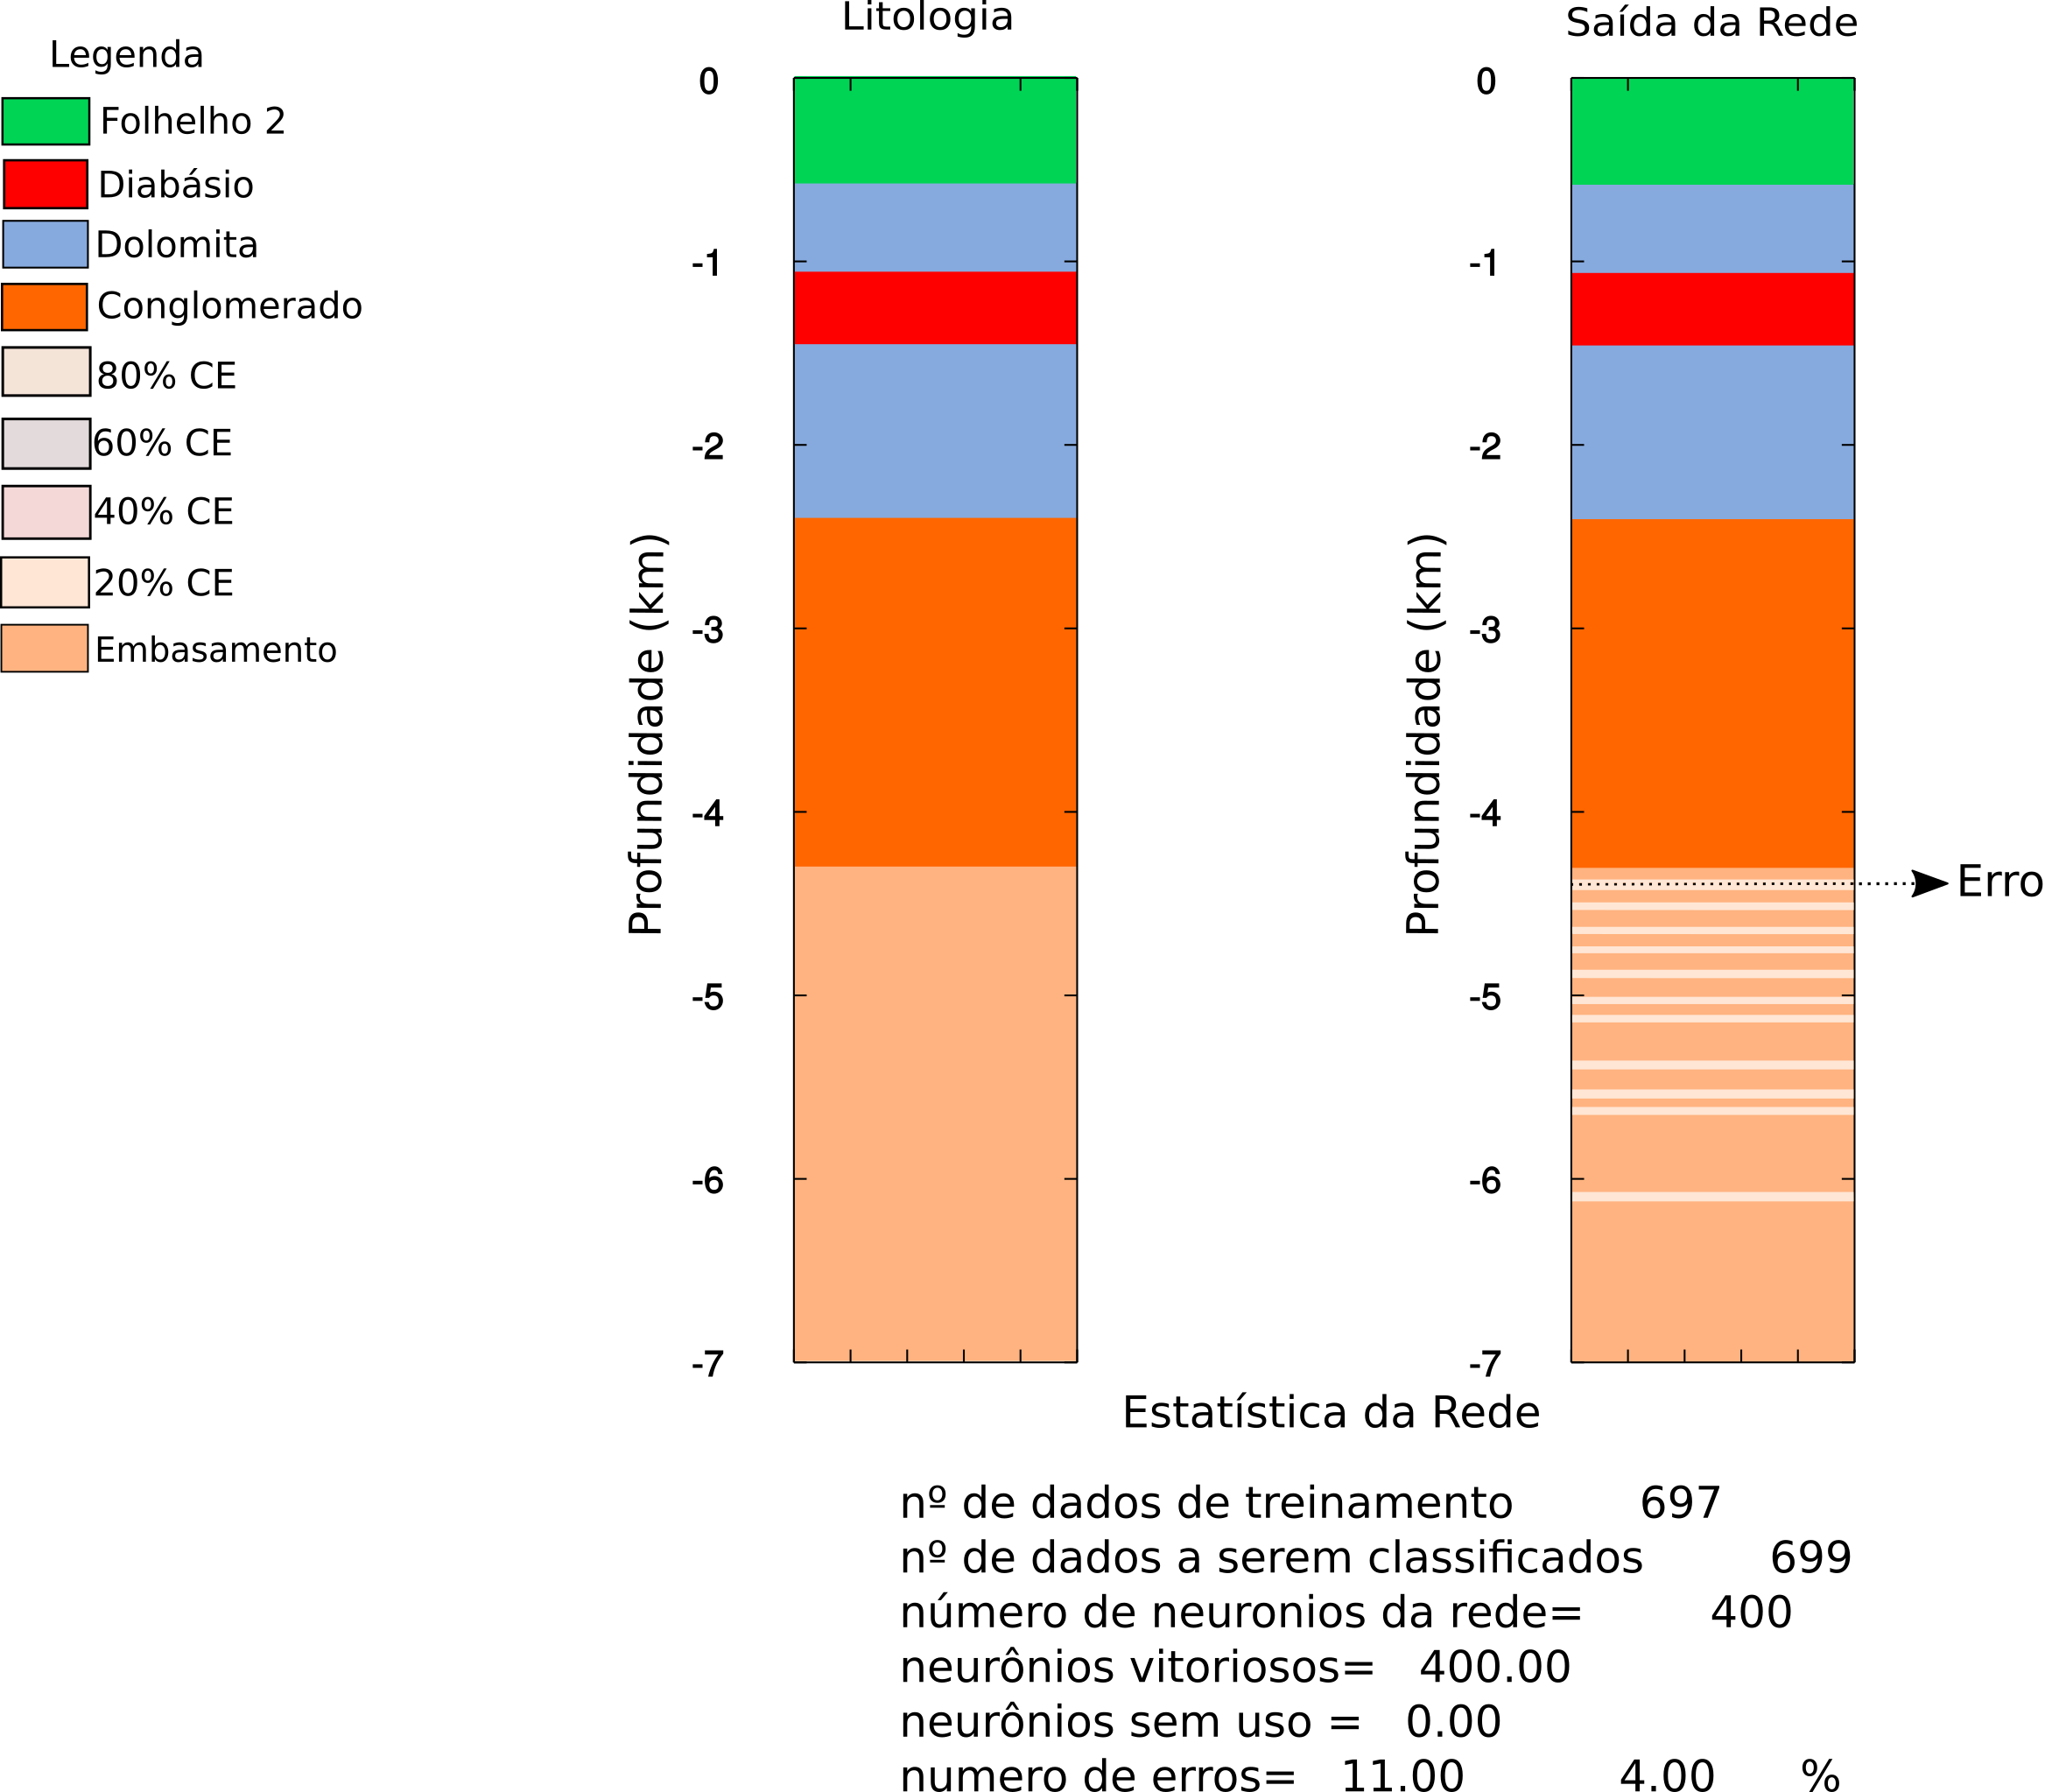
\includegraphics[scale=0.6]{Imagens/IDT1.png}
	}
	\caption{Dado de saída da rede para o poço de classificação C1.}
	\label{convergencia}
\end{figure} 





\begin{figure}[H]
	\centering
	\setlength{\fboxsep}{8pt}
	\setlength{\fboxrule}{0.1pt}
	\fbox{
		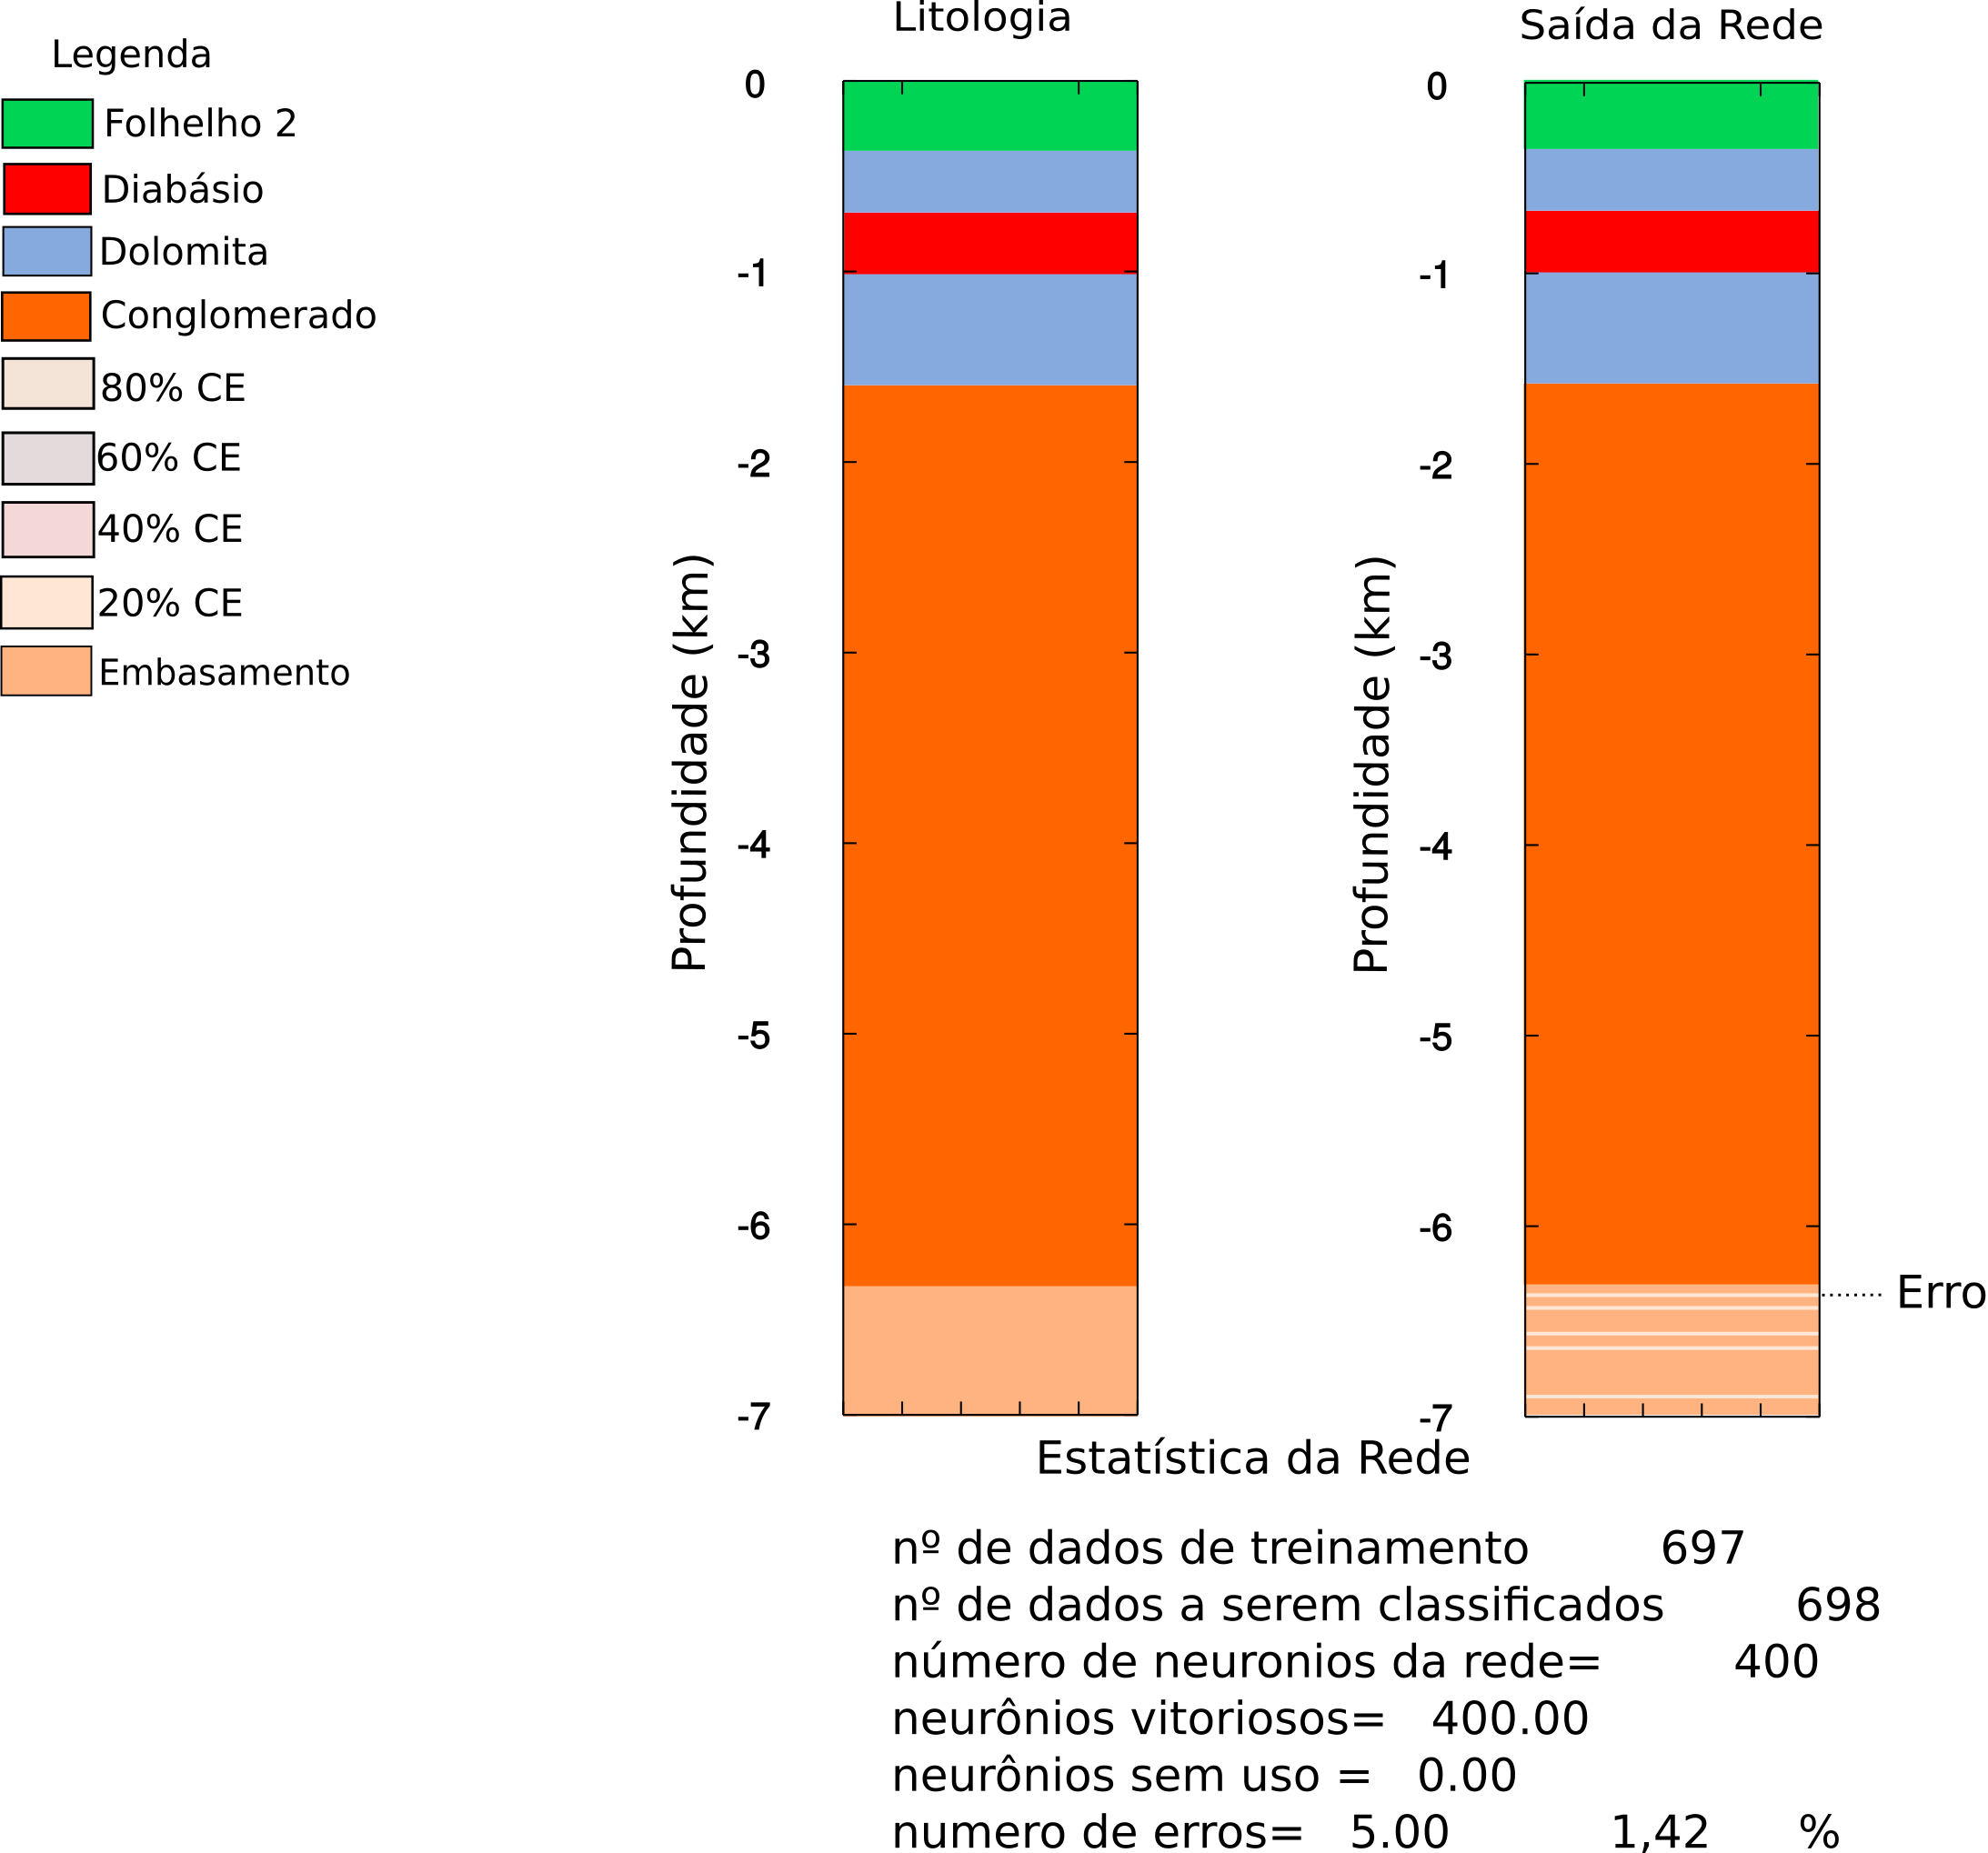
\includegraphics[scale=0.6]{Imagens/IDC2.png}
	}
	\caption{Dado de saída da rede para o poço de classificação C2.}
	\label{convergencia}
\end{figure} 



  \chapter{Conclusões}

O teste de convergência da rede, Fig \ref{convergencia}, realizado durante a etapa de treinamento, indicou que o número de erros não iria diminuir após o milésimo ciclo de treinamento. Sendo o resultado, Fig. \ref{SOM}, deste teste usado como parâmetro para o número de repetições realizadas para os casos de identificação da rede. 

Os diagramas de velocidades por densidade e o de velocidade por raio-gama, Fig. \ref{clusterT1}, Fig. \ref{clusterC1} e Fig. \ref{clusterC2}, apresentaram os agrupamentos mais bem separados. Portanto estas propriedades físicas (densidade, velocidade e raio-gama) tem uma importância relativa maior ,na classificação das litologias dos poços C$1$ e C$2$. 

A saída da rede aponta que o maior caso de erros ocorreram em uma única classe de rocha, a do embasamento. Esses erros fizeram com que conglomerados fossem classificados como rochas do embasamento, nos dois casos dos poços de classificação, o poço C$1$ e o poço C$2$.  Uma das razões pode ser o fato das misturas de conglomerado e embasamento serem finas demais para a rede conseguir realizar uma identificação de padrão. Ou pelo fato dos conjuntos de propriedades físicas da mistura de $20\%$ se aproximar das propriedades físicas que representam o litotipo embasamento. 

O menor número de erros relativos encontrados, no poço C$2$, Fig. \ref{Class C2}, deve-se a escolha da alocação do furo, no perfil. O poço C$2$ localiza-se em um baixo estrutural, atingindo menos de $1$km do embasamento. Entretanto, o poço C$1$, Fig. \ref{Class C1}, encontra-se em um alto estrutural, divergindo do poço C$2$ e produzindo, consequentemente, os maiores erros relativos encontrados.    




  \backmatter

  % estilo de citações por ordem alfabética (defaut da classe ONTeX)
  %\bibliographystyle{apalike}
  \bibliographystyle{on-plain}
  \bibliography{references}

  \appendix
  % A linha "\include" abaixo inclui um capítulo de apêndice.
  % Edite o arquivo "appenA.tex" de acordo com as suas necessidades.
  % É possível incluir outros capítulos de apêndice. Para tanto,
  % crie outros arquivos "appenX.tex", de acordo com as suas necessidades,
  % e inclua-os no documento utilizando "\include{appenX}".
  %\chapter{Cronograma de Atividades}

%\begin{figure}[H]
%	\centering
%	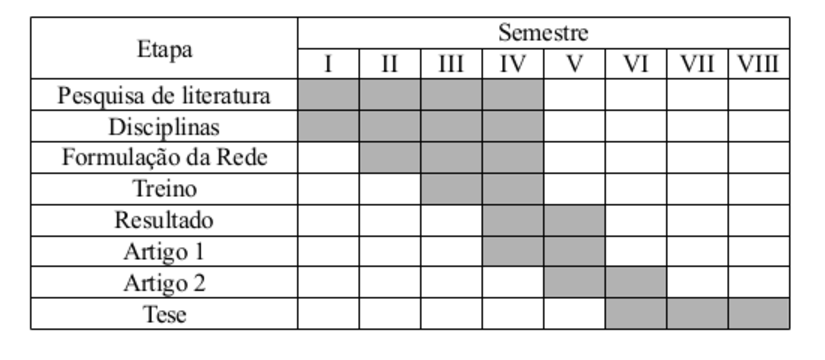
\includegraphics[height=6.5cm, width=16cm]{Imagens/Cronograma.pdf}
%	\caption{Cronograma previsto para o projeto.}
%\end{figure}


\begin{table}[H]
\centering
%\flushleft

% definindo o tamanho da fonte para small
% outros possíveis tamanhos: footnotesize, scriptsize
\begin{small}

% redefinindo o espaçamento das colunas
\setlength{\tabcolsep}{3pt}

% \cline é semelhante ao \hline, porém é possível indicar as colunas que terão essa a linha horizontal
% \multicolumn{10}{c|}{Meses} indica que dez colunas serão mescladas e a palavra Meses estará centralizada dentro delas.
\rotatebox{90}{
\begin{tabular}{|c|c|c|c|c|c|c|c|c|c|c|c|c|c|c|c|c|c|c|c|c|c|c|c|c|}\hline
 & \multicolumn{24}{c|}{Meses}\\ \cline{2-25}
\raisebox{1.5ex}{Etapa} & 01 & 02 & 03 & 04 & 05 & 06 & 07 & 08 & 09 & 10 & 11 & 12 & 13 & 14 & 15 & 16 & 17 & 18 & 19 & 20 & 21 & 22 & 23 & 24 \\ \hline

Pesquisa na Literatura & X & X & X & X & X & X & X & X & X & X & X & X & X & X & X & X & X & X & X & X & X & X & X & X\\ \hline
Disciplinas & & & X & X & X & X & X & X & X & X & X & X & & & X & X & X & X & X & X & X & X & X & X \\ \hline
Formulação da Rede & & & & & & & & X & X & X & X & X & X & X & X & X & X & & & & & & & \\ \hline
Treino & & & & & & & & & & & & & X & X & X & X & X & X & X & X & X & X & X & X \\ \hline
Resultado & & & & & & & & & & & & & & & & & & & & X & X & X & X & X \\ \hline
Artigo 1 & & & & & & & & & & & & & & & & & & & & & & & X & X \\ \hline
Artigo 2 & & & & & & & & & & & & & & & & & & & & & & & & \\ \hline
Tese & & & & & & & & & & & & & & & & & & & & & & & & \\ \hline
\end{tabular}
}
\end{small}
\caption{Cronograma das atividades previstas para o primeiro biênio}
\label{t1_cronograma}
\end{table}


\begin{table}[H]
\centering

% definindo o tamanho da fonte para small
% outros possíveis tamanhos: footnotesize, scriptsize
\begin{small}

% redefinindo o espaçamento das colunas
\setlength{\tabcolsep}{3pt}

% \cline é semelhante ao \hline, porém é possível indicar as colunas que terão essa a linha horizontal
% \multicolumn{10}{c|}{Meses} indica que dez colunas serão mescladas e a palavra Meses estará centralizada dentro delas.
\rotatebox{90}{
\begin{tabular}{|c|c|c|c|c|c|c|c|c|c|c|c|c|c|c|c|c|c|c|c|c|c|c|c|c|}\hline
 & \multicolumn{24}{c|}{Meses}\\ \cline{2-25}
\raisebox{1.5ex}{Etapa} & 25 & 26 & 27 & 28 & 29 & 30 & 31 & 32 & 33 & 34 & 35 & 36 & 37 & 38 & 39 & 40 & 41 & 42 & 43 & 44 & 45 & 46 & 47 & 48 \\ \hline

Pesquisa na Literatura & X & X & X & X & X & X & & & & & & & & & & & & & & & & & & \\ \hline
Disciplinas & & & & & & & & & & & & & & & & & & & & & & & & \\ \hline
Formulação da Rede & & & & & & & & & & & & & & & & & & & & & & & & \\ \hline
Treino & & & & & & & & & & & & & & & & & & & & & & & & \\ \hline
Resultado & & X & X & X & X & X & X & X & & & & & & & & & & & & & & & & \\ \hline
Artigo 1 & & X & X & X & & & & & & & & & & & & & & & & & & & & \\ \hline
Artigo 2 & & & & & X & X & X & X & X & & & & & & & & & & & & & & & \\ \hline
Tese & & & & & & & & & & & & & & & X & X & X & X & X & X & X & & & \\ \hline

\end{tabular}
}
\end{small}
\caption{Cronograma das atividades previstas para o segundo biênio}
\label{t2_cronograma}
\end{table}


\end{document} 